%%%% ijcai11.tex

\typeout{IJCAI-11 Instructions for Authors}

% These are the instructions for authors for IJCAI-11.
% They are the same as the ones for IJCAI-07 with superficical wording
%   changes only.

\documentclass{article}
% The file ijcai11.sty is the style file for IJCAI-11 (same as ijcai07.sty).
\usepackage{ijcai11}
\usepackage{mathtools}
\usepackage[utf8]{inputenc}
\usepackage{amsmath}
\usepackage{slashbox}

% For importing images.
\usepackage{graphicx}

% The language we want and appropriate hyphenation.
\usepackage[dutch]{babel}

% Hyphenation rules.
\hyphenation{biopotentiaal-schommelingen}

% Use the postscript times font!
\usepackage{times}

% the following package is optional:
%\usepackage{latexsym} 


\title{Kijkrichtingen detecteren door middel van elektromyografie}
\author{Kevin Boets \\ Katholieke Universiteit Leuven\\ Departement Computerwetenschappen \\ kevin.boets@student.kuleuven.be
\And
Gertjan Franken \\ Katholieke Universiteit Leuven\\ Departement Computerwetenschappen \\ gertjan.franken@student.kuleuven.be}

\begin{document}

\maketitle

\begin{abstract}
In de zoektocht naar natuurlijke user interfaces gebeurt er onderzoek naar besturing door middel van de ogen. In deze paper wordt gebruik gemaakt van EMG (Elektromyografie) signalen om eenvoudige oogbewegingen te detecteren. Hiervoor onderzoeken we twee verschillende methodes: thresholds en patronen. In deze tekst bespreken en vergelijken we beide methodes uitvoerig. [TODO conclusie zin?]
\end{abstract}

\section{Introductie}

Reeds verschillende manieren om oogbewegingen te detecteren zijn bedacht. Zo kan men al door middel van camera's de ogen volgen. Hierbij gaat men op zoek naar de positie van de iris om de stand van het oog te achterhalen. Deze technieken zijn al ver ontwikkeld, maar bieden nog geen oplossing voor alle problemen. Daarom onderzoeken wij een andere manier. We maken gebruik van sensoren die rond de ogen zijn aangebracht, om elektromyografie (EMG) signalen te meten. Aan de hand van deze signalen proberen we te achterhalen in welke richting de gebruiker kijkt. Als invoer krijgen we twee elektrooculogrammen die respectievelijk de kijkrichtingen links-rechts en boven-onder voorstellen. Figuur~\ref{fig:originaldata} geeft een mooi voorbeeld weer van het elektrooculogram betreffende de kijkrichtingen links en rechts. Hierbij stellen de dalen de kijkrichting links voor en stellen de bergen de kijkrichting rechts voor.

\section{Preprocessing}

Het signaal dat we krijgen doorgestuurd, afkomstig van de sensoren, is zeer ruw. Om hier kijkrichtingen uit af te kunnen leiden, gaan we de data eerst beter leesbaar maken. Dit is de preprocessing-stap. Deze stap voeren we uit op elke dataset,  alvorens we deze gaan analyseren. Beschouw de data in figuur~\ref{fig:originaldata} als de originele data.

\begin{figure}[h]
\centering
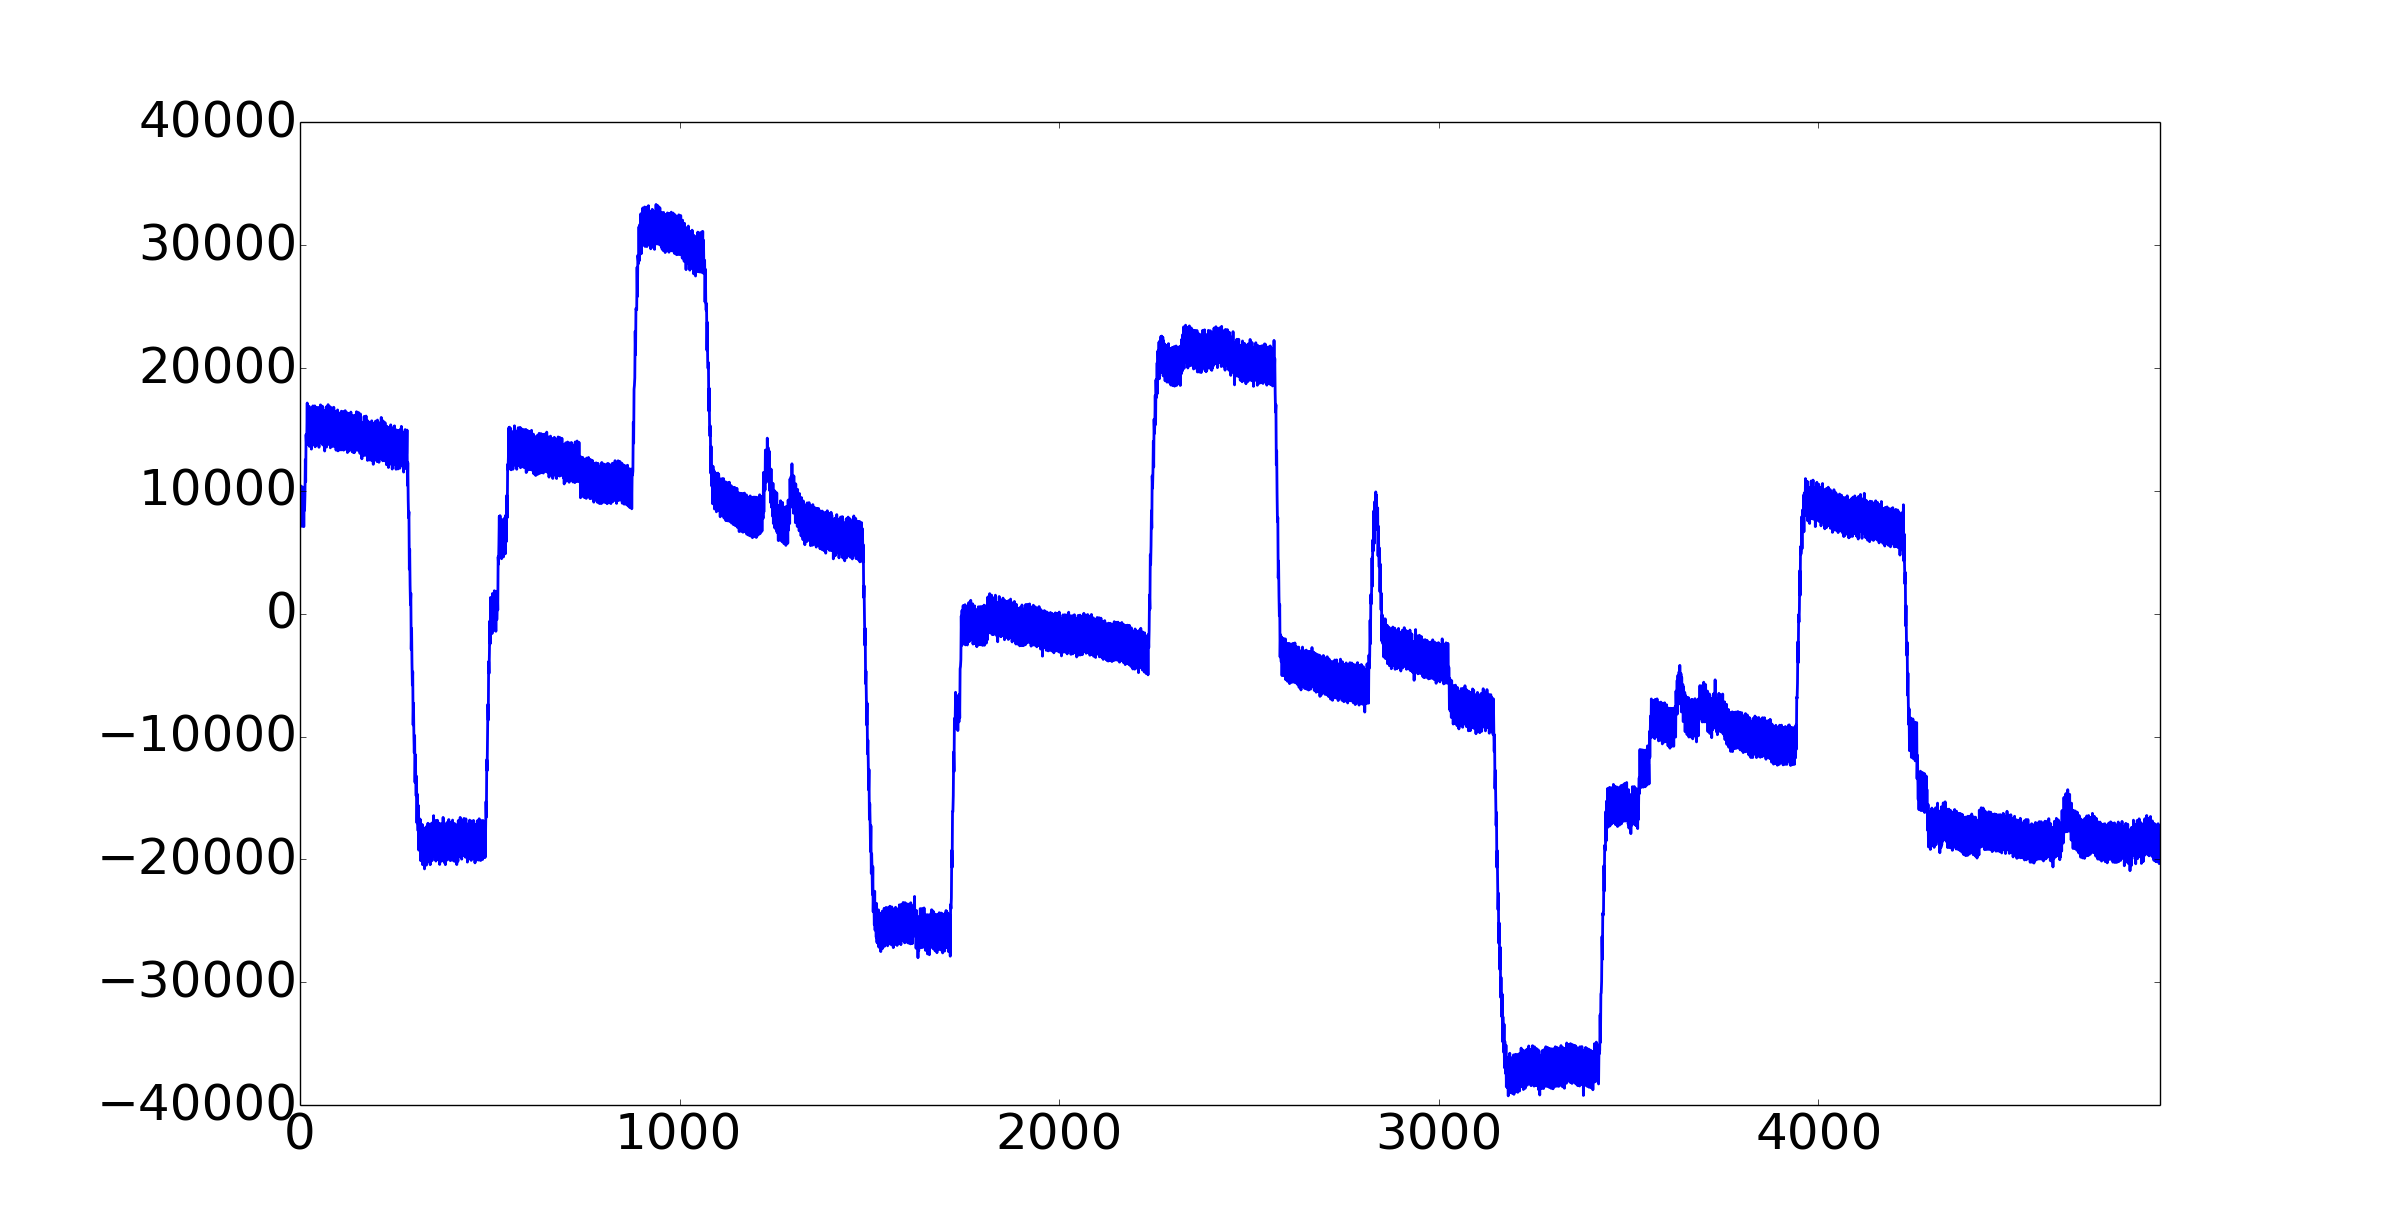
\includegraphics[width=\linewidth]{images/original_data}
\caption{Originele data rechtstreeks afkomstige van de hardware. De grootheid op de x-as is tijd en op de y-as is dit het voltage.}
\label{fig:originaldata}
\end{figure}

Als eerste gaan we de ruis en knipperingen zo goed mogelijk proberen te verminderen. Dit gebeurt door middel van een low-pass filter. Deze filter verzacht het signaal door de hoogfrequentie te verminderen. Hiervoor gebruiken we de butterworth filter van SciPy voor Python. Door met de parameters van deze filter te experimenteren, probeerden we een optimale filtering te vinden voor het originele signaal. Uit de uiteindelijk gekozen parameters, berekenen we dan de cutoff frequenty $cf$ zoals in vergelijking~\ref{eq:cutoff} staat beschreven. Alle frequenties hoger dan deze $cf$ zullen worden afgezwakt. In deze vergelijking staat $sf$ voor de sampling frequentie, dit geeft aan hoe snel datapunten doorgestuurd worden door de sensoren. $Wn$ staat voor de genormaliseerde cutoff frequentie. Aan de hand van de gevonden cutoff frequentie $cf_1$, filteren we de ruis en knipperingen. Dit gebeurt in vergelijking~\ref{eq:ruisfiltering}, waarbij $s$ het originele signaal is. Omdat $sf_1$ bij ons gelijk is aan 2 Hz en $Wn_1$ gelijk is aan 0,05, komen we uit op een waarde van 0,625 Hz voor $cf_1$.

\begin{equation}
\label{eq:cutoff}
cf = \frac{fs \cdot Wn}{2}
\end{equation}

\begin{equation}
\label{eq:ruisfiltering}
s' = lowpass(s, cf_1)
\end{equation}

Daarna focussen we ons op de biopotentiaalschommelingen. Deze schommelingen kunnen we niet op voorhand voorspellen en verschillen van persoon tot persoon. Als we deze schommelingen kunnen verminderen, kunnen we meer steunen op absolute waarden van het signaal. In dit tweede deel van de preprocessing-stap gebruiken we opnieuw een low-pass filter. Deze keer gebruiken we een lage cutoff frequentie $cf_2$ met de waarde [TODO]. Na deze filtering van de data, blijven enkel de signalen met een lage frequentie over. Het resultaat is de benadering van de biopotentiaal van de gebruiker die doorheen de tijd fluctueert. We kunnen nu de biopotentiaalschommelingen uit onze originele data verminderen door de gevonden benadering hiervan af te trekken, zoals in vergelijking~\ref{eq:aftrekkingbiopotentiaal}. De schommelingen verdwijnen niet volledig, maar worden wel sterk verminderd. Figuur~\ref{fig:filtereddata} stelt het resultaat van de besproken filtereringen voor.

\begin{equation}
\label{eq:aftrekkingbiopotentiaal}
s'' = s' - lowpass(s', cf_2)
\end{equation}

Bij veelvuldige herhaling van dezelfde kijkrichting, wordt een probleem in verband met deze methode zichtbaar. Als er veel en opeenvolgend naar éénzelfde richting gekeken wordt, zullen de waarden in de data algemeen lager of hoger zijn. De gefilterde data zal hierdoor ook algemeen lager of hoger liggen. Dit is een probleem aangezien het de benadering van de biopotentiaal moet voorstellen. Doordat de gevonden benadering foutief is, zullen ook alle volgende bewerkingen een incorrecte uitkomst hebben. Wanneer we dus deze benadering aftrekken van de oorspronkelijke data, zal de data ongewenst verschuiven volgens de y-as. Deze verschuiving illustreren we in figuur~\ref{fig:bio_fout}.   Hierdoor zal het werken met absolute waarden slechte resultaten opleveren. Omdat de gebruiker zelf kiest welke reeks van kijkrichtingen hij uitvoert, kunnen we deze situatie niet vermijden. We willen dan ook een oplossing vinden voor wanneer we de absolute waarden nodig hebben.

\begin{figure}[h]
\centering
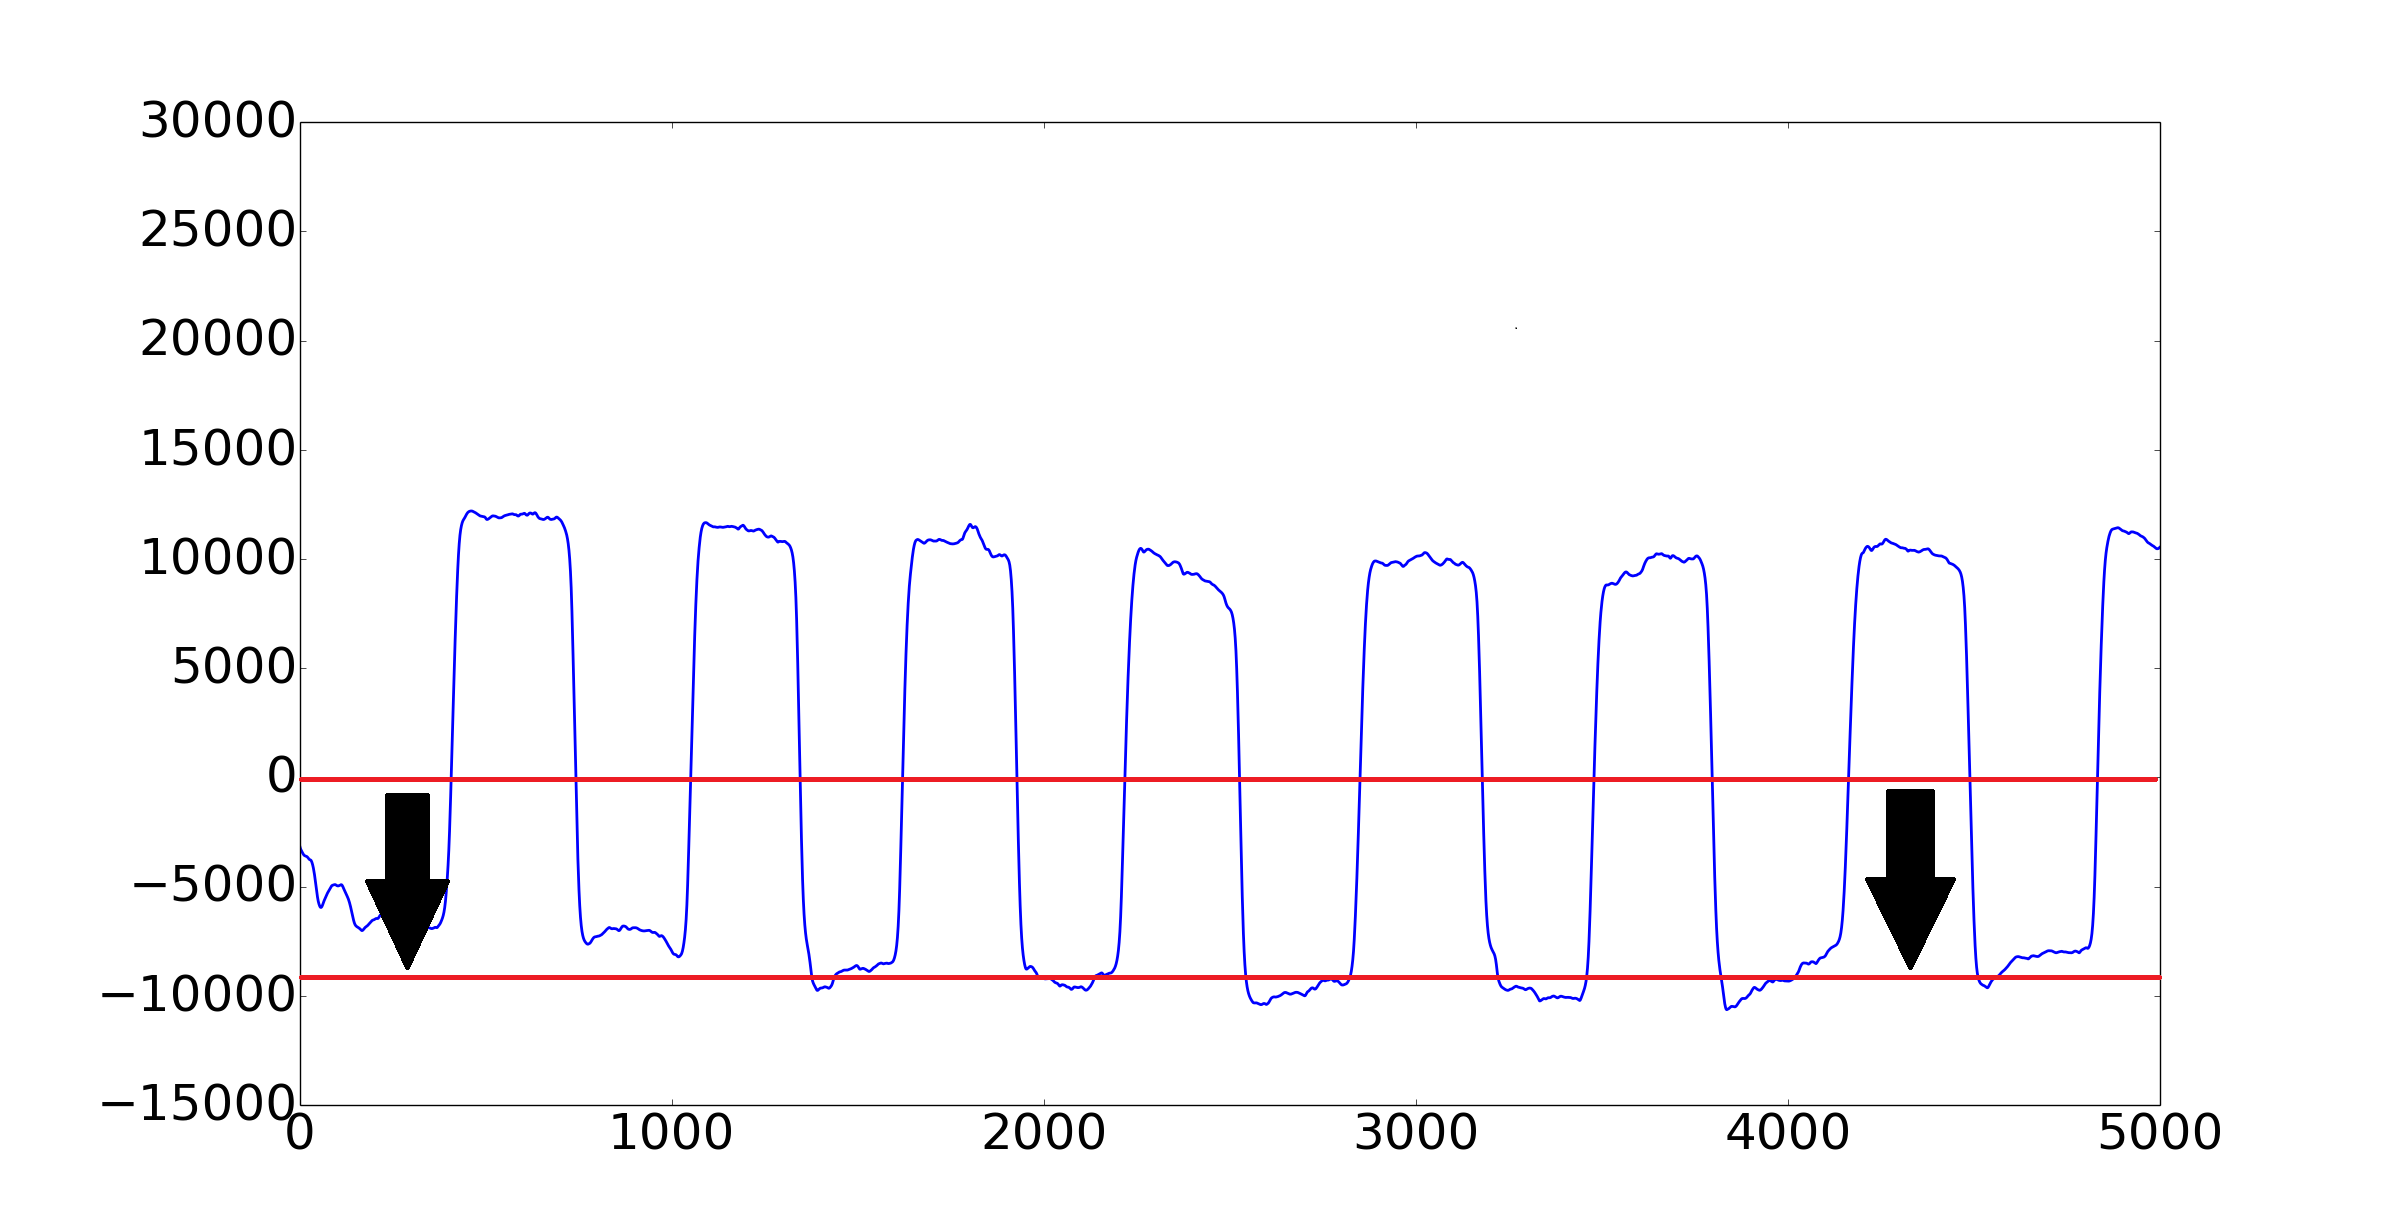
\includegraphics[width=\linewidth]{images/biofout}
\caption{Na aftrek van de foutieve benadering van de biopotentiaal, zien we dat de waardes ongewenst naar onder zijn gegaan. Hierdoor is rechtdoor kijken niet meer rond de $y = 0$ lijn, maar wel veel lager rond de $y = -10000$ lijn.}
\label{fig:bio_fout}
\end{figure}

\begin{figure}[h]
\centering
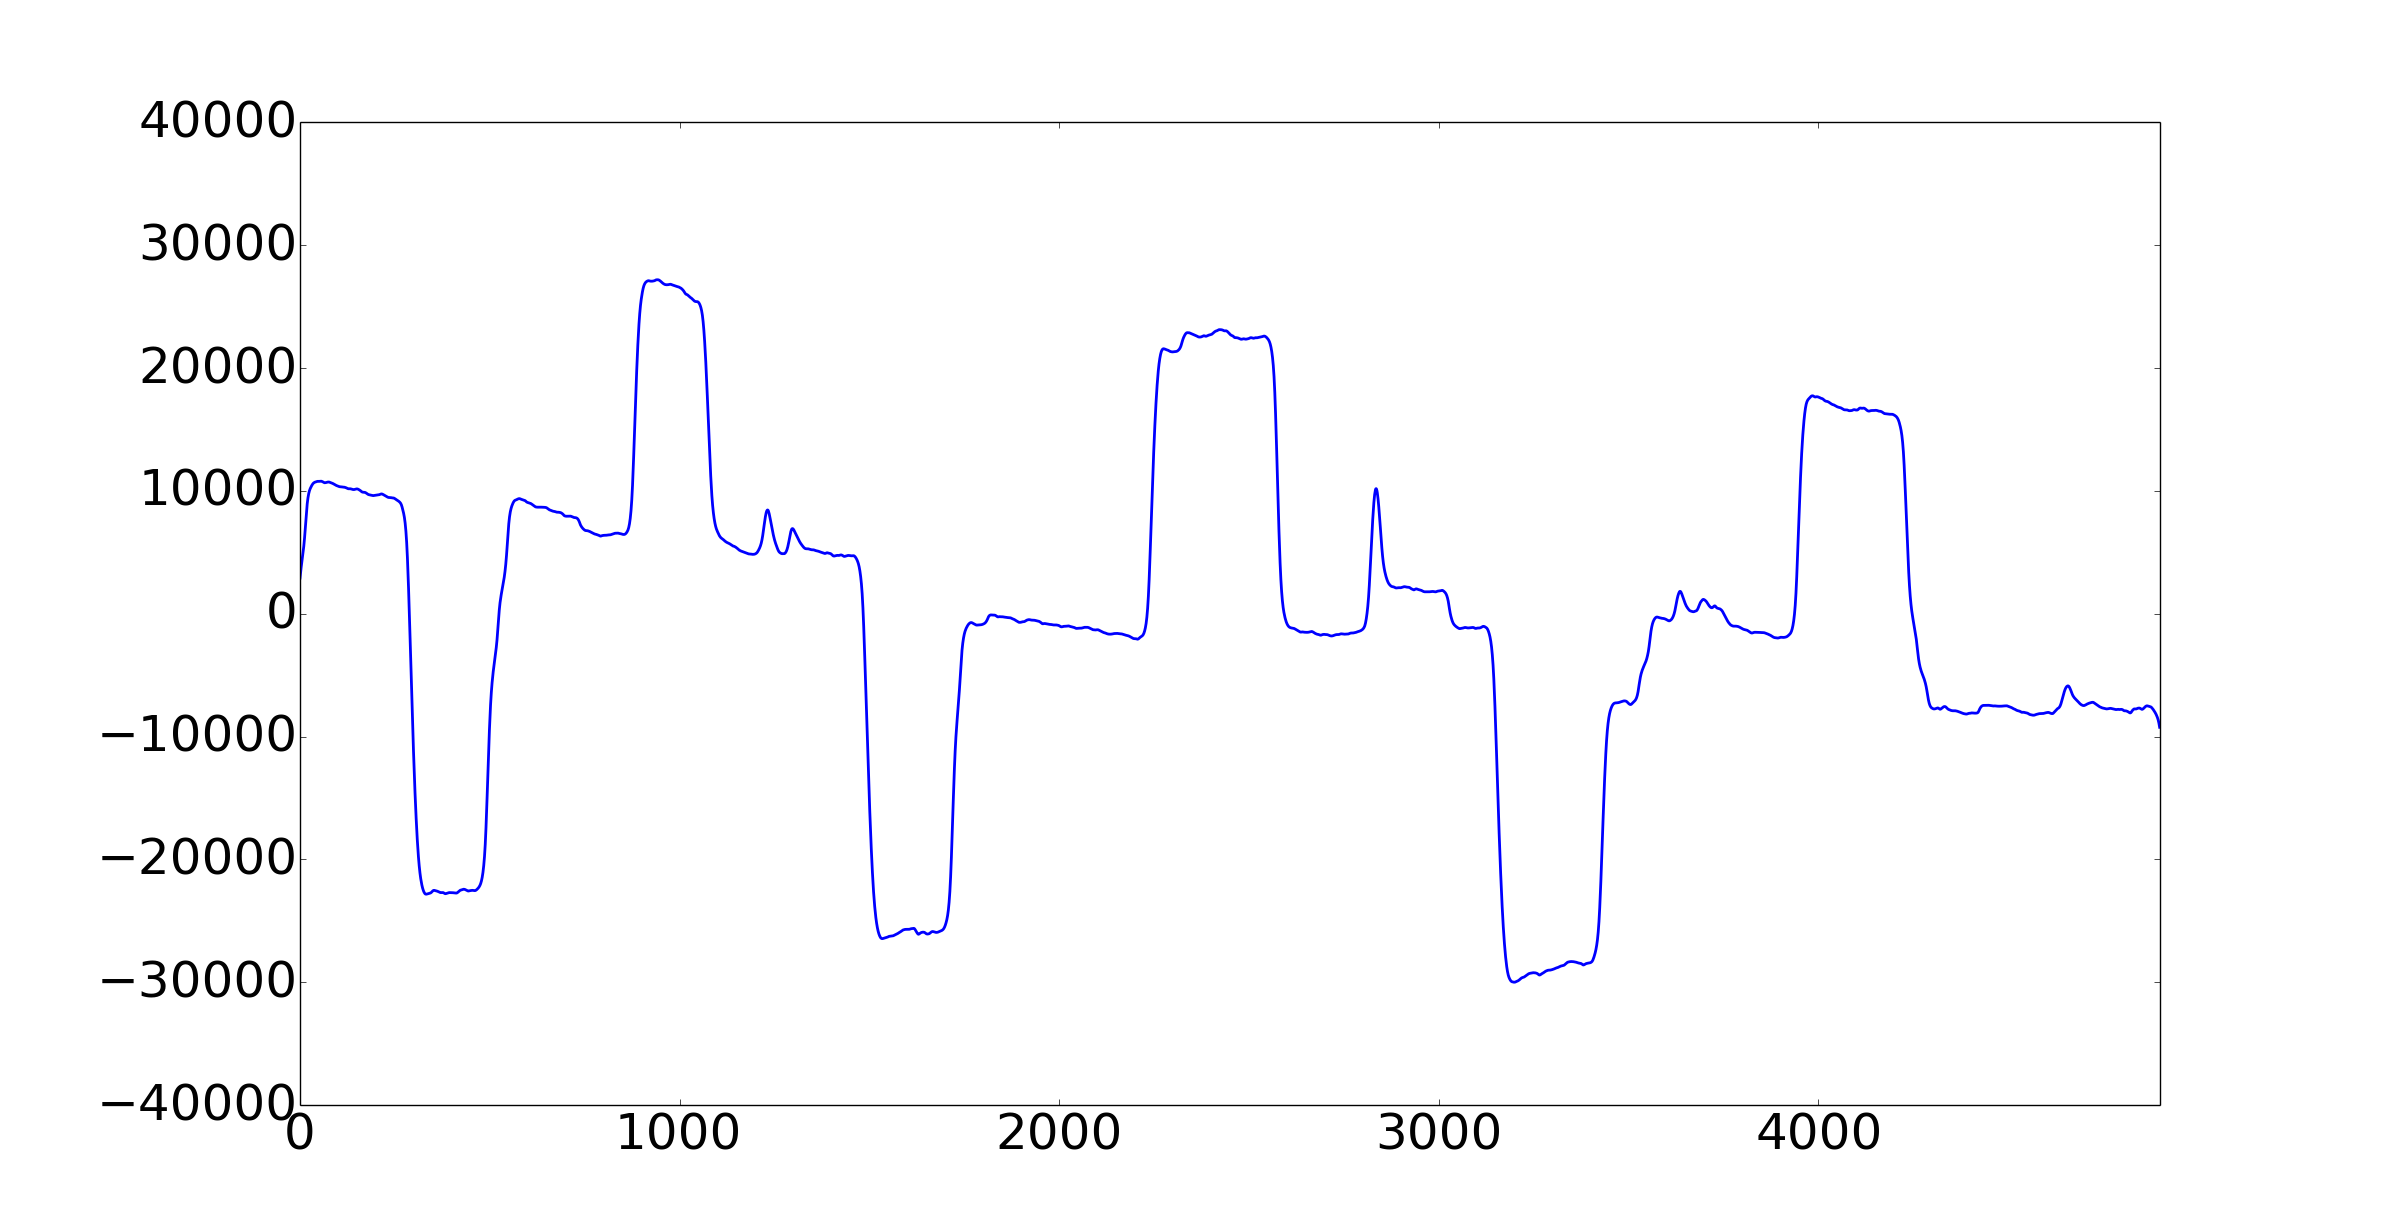
\includegraphics[width=\linewidth]{images/filtered_data}
\caption{Het resultaat van de twee filteringen op de originele data. De ruis is sterk verminderd en de sterkte van de knipperingen is afgenomen. De biopotentiaalschommeling is niet helemaal weg, maar wel voldoende verminderd.}
\label{fig:filtereddata}
\end{figure}



Na toepassing van de vorige filteringen, discretiseren we de data. Deze stap is eerder optioneel en wordt enkel in de methode met patronen gebruikt. Het grote voordeel van deze stap is dat we minder berekeningen zullen moeten doen, wat de uitvoeringstijd van het programma ten goede komt. Hiervoor gebruiken we de SAX-discretisatie (Symbolic Aggregate approXimation) \cite{sax}. Eerst wordt de data genormaliseerd. We definiëren op voorhand hoeveel waarden een letter voor moet stellen. Dit is de constante $w$. De data die we willen discretiseren, verdelen we op in partities van lengte $w$. Elke partitie zal een bepaalde letter krijgen, afhankelijk van zijn gemiddelde. Het aantal verschillende letters dat we gebruiken, hangt af van de alfabetgrootte $a$. Volgens de normale verdeling wordt nu elke partitie aan een letter gekoppeld. Zie figuur~\ref{fig:discretization} voor de visuele werking. Eigenlijk stelt elke letter nu een reeks van waarden voor. Om SAX-woorden voor te kunnen stellen in grafieken, geven we elke letter ook een waarde. Dit is het gemiddelde van de intervalgrenzen die de letter op zicht neemt.

\begin{figure}[h]
\centering
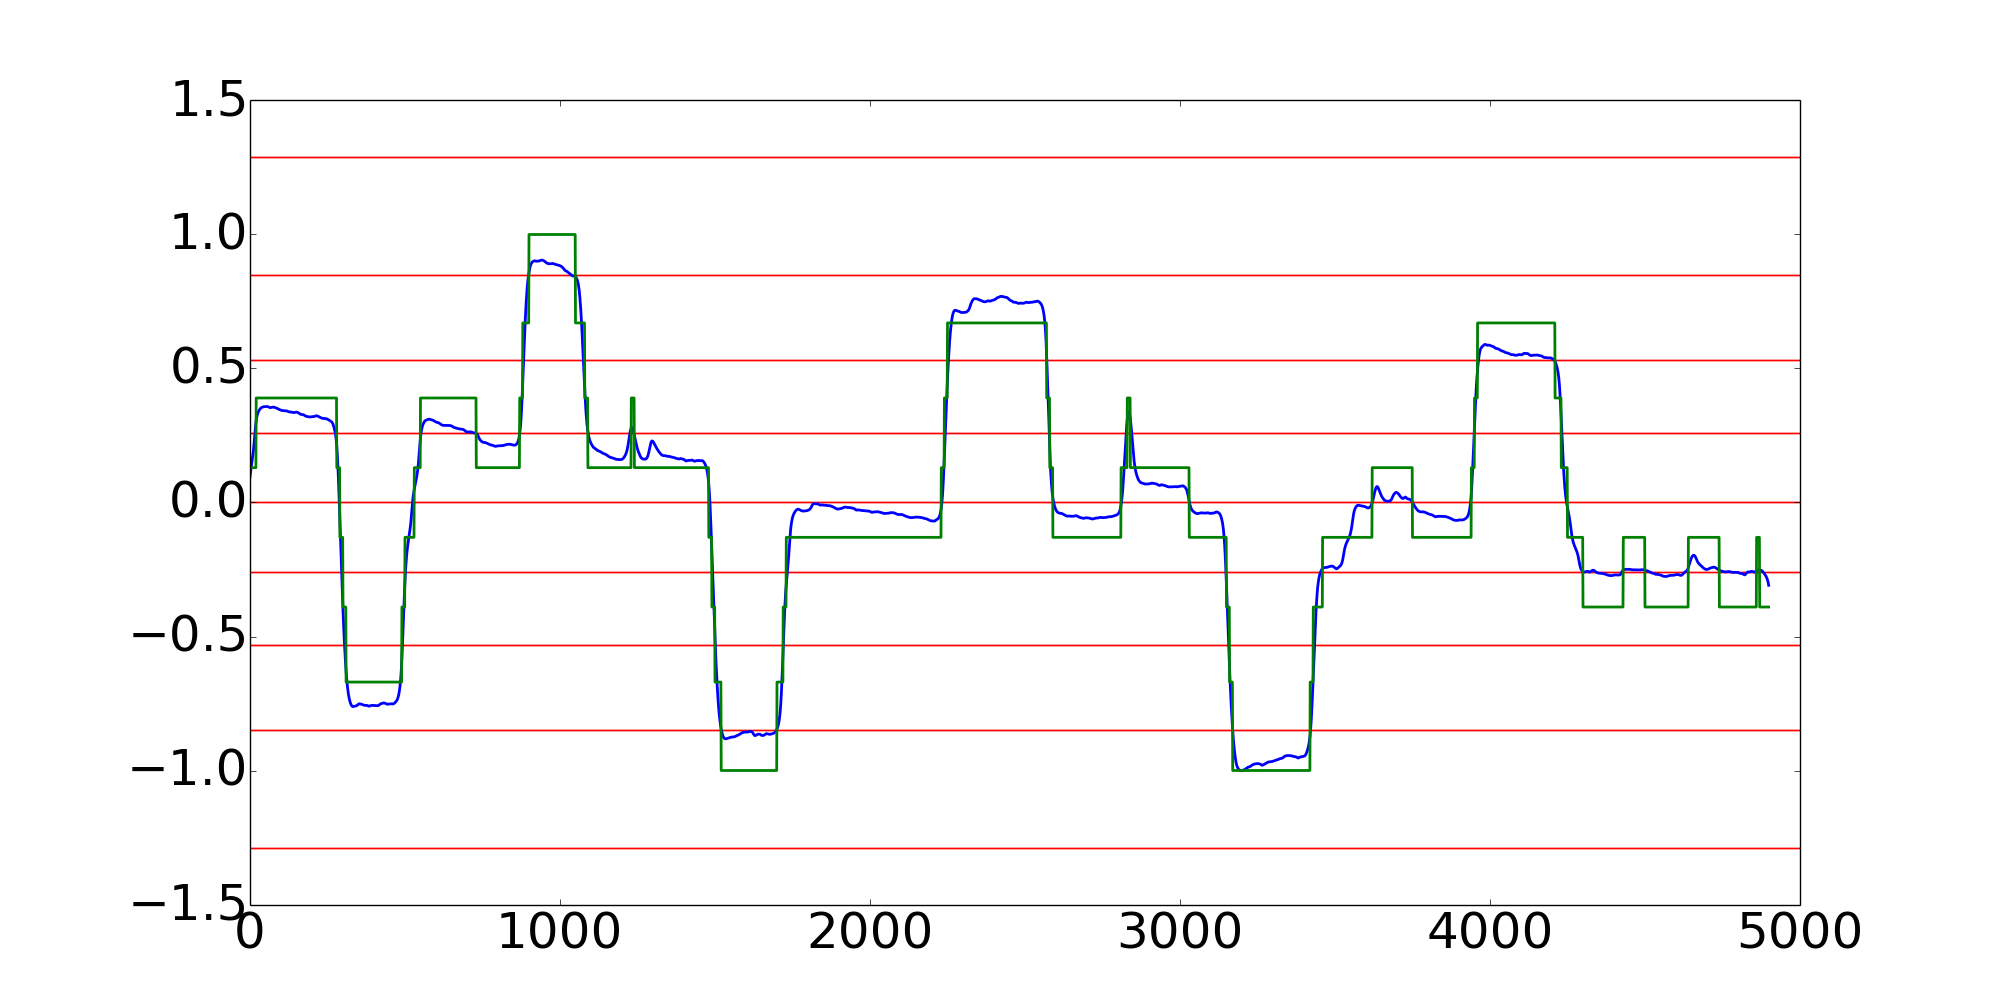
\includegraphics[width=\linewidth]{images/sax_normaal_verdeling}
\caption{De groene lijn stelt de discretisatie voor van de gefilterde data die in het blauw staat. De rode horizontale lijnen geven de distributie weer van de SAX-letters. Deze distributie is volgens de normale verdeling met gemiddelde 0 en standaarddeviatie 1.}
\label{fig:discretization}
\end{figure}

\section{Gebruikte methoden}

In ons onderzoek hebben we gebruik gemaakt van twee verschillende methoden om kijkrichtingen te herkennen. Deze methoden steunen respectievelijk op thresholds en patronen. Beide methoden beginnen met een calibratie-fase, gevolgd door een herkennings-fase. In de calibratie-fase laten we de gebruiker naar een aantal richtingen kijken, waarna we deze data analyseren. De gevonden informatie koppelen we aan de juiste kijkrichting. In de herkennings-fase wordt deze informatie gebruikt om in de nieuwe data kijkrichtingen te detecteren.

\subsection{Thresholds}

De eenvoudigste methode is de methode gebruikmakend van thresholds. Het steunt vooral op de absolute waarden van de data. Het basis idee van deze methode is als volgt. Er wordt een bovengrens gedefinieerd voor elke kijkrichting in de calibratie-fase. Als deze overschreden wordt in de herkennings-fase, gaan we er van uit dat er in de overeenkomstige kijkrichting gekeken wordt.

In de calibratie-fase wordt aan de gebruiker gevraagd om een bepaalde sequentie van kijkrichtingen uit te voeren. Vervolgens voeren we de preprocessing-stap uit in verband met de ruis, knipperingen en biopotentiaal. Hier maken we geen gebruik van de SAX-discretisatie omdat deze methode al efficiënt genoeg is. De preprocessed dataset gebruiken we dan om goede bovengrenzen te vinden. Figuur~\ref{fig:thresholds} illustreert een voorbeeld van welke bovengrenzen gebruikt kunnen worden op het signaal dat we eerder al hadden besproken.

\begin{figure}[h]
\centering
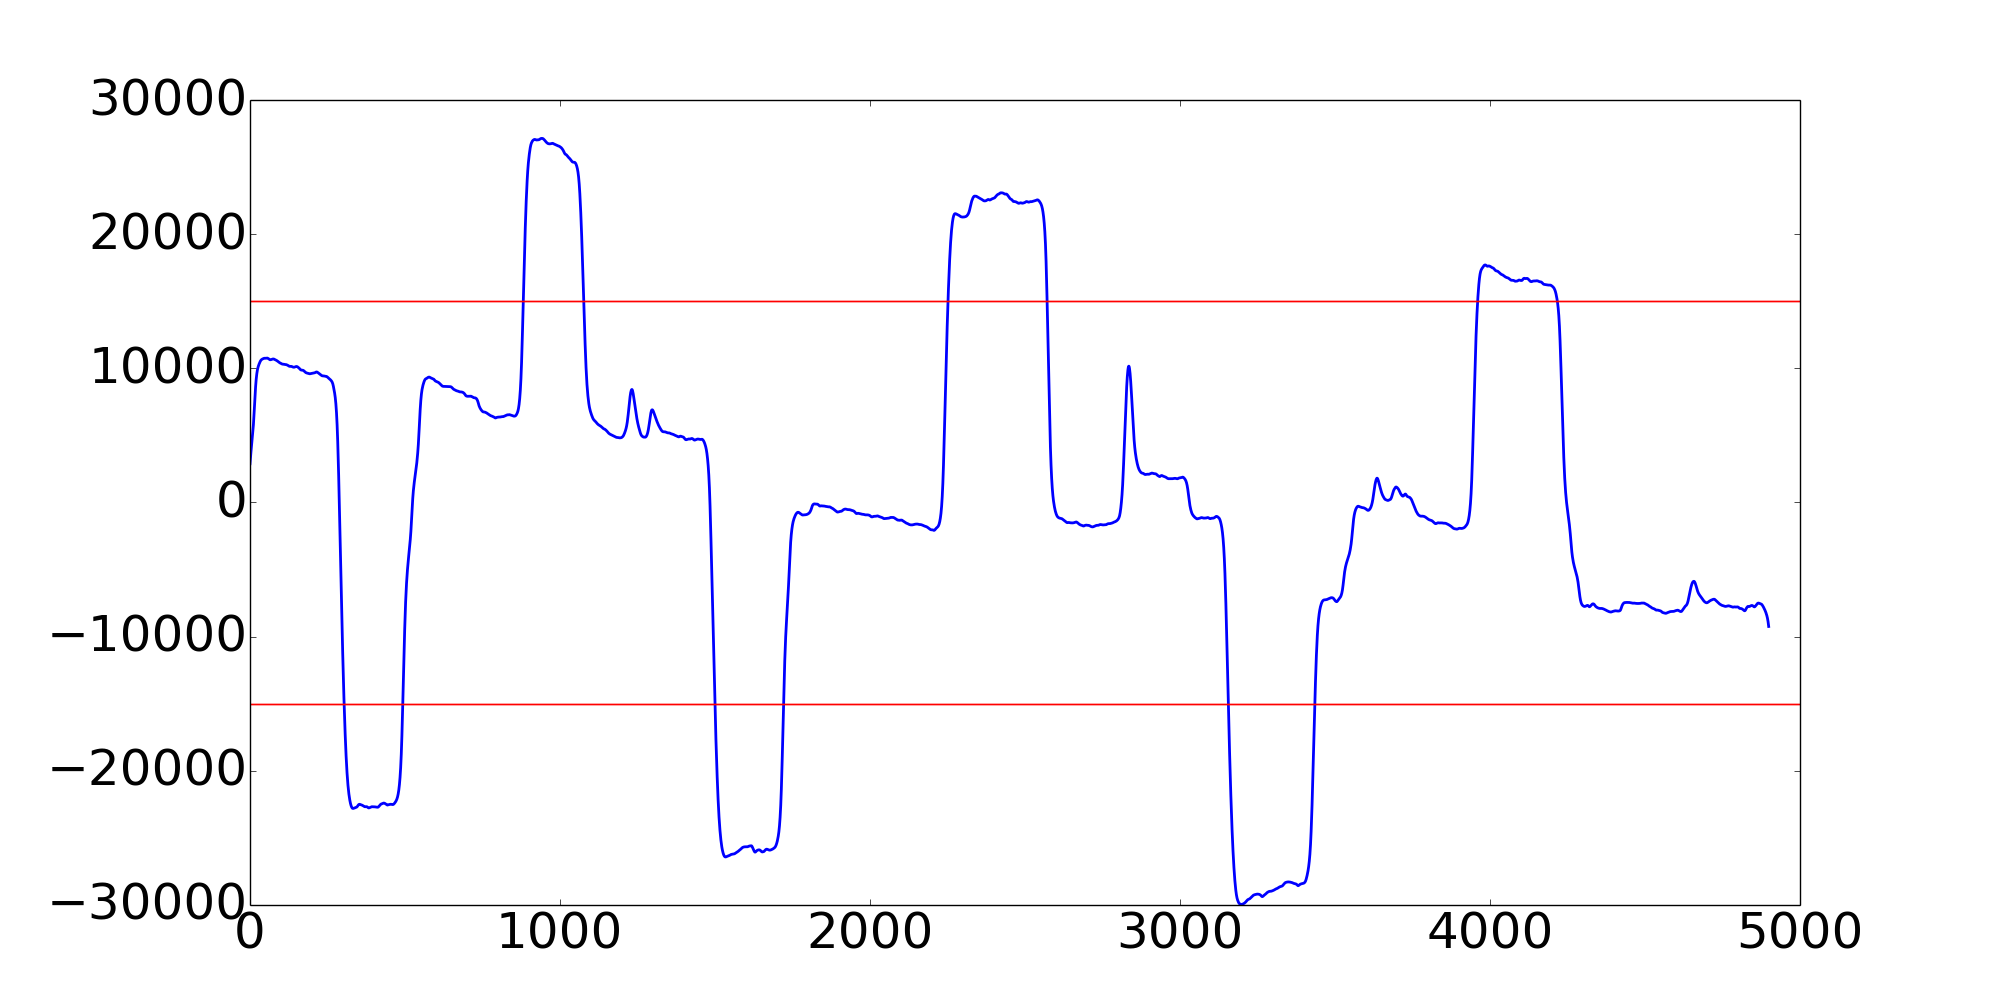
\includegraphics[width=\linewidth]{images/thresholds_voorbeeld}
\caption{In deze afbeelding stellen de rode horizontale lijnen mogelijke bovengrenzen voor.}
 \label{fig:thresholds}
\end{figure}

Eens we de bovengrenzen hebben gevonden, kunnen we deze in de herkennings-fase gebruiken om kijkrichtingen te detecteren. Om deze gevonden bovengrenzen te kunnen gebruiken, zullen we eerst dezelfde preprocessing stappen utivoeren op de nieuwe data. Belangrijk is dat we het signaal ten allen tijde stabiel houden, we werken immers met absolute waarden.

Om kijkrichtingen te detecteren, gaan we de bovengrenzen vergelijken met de waardes uit de data. Wanneer een bovengrens overschreden wordt, toont dit aan dat de gebruiker mogelijk in een van de richtingen aan het kijken is. Dit kunnen we echter niet zomaar aannemen. Een enkele piek, zoals een knippering, zou dan ook ongewild worden herkend als kijkrichting. Om voor meer zekerheid te zorgen, wachten we tot dezelfde grens opeenvolgend meerdere keren overschreden is. Hoeveel keren definiëren we op voorhand. Het aantal dat we kiezen is een afweging tussen detectiekans en zekerheid. Bij een klein aantal is de kans op detectie hoog, maar zijn we minder zeker over de geldigheid van de detectie. Een groot aantal zal anderzijds veel zekerheid verschaffen, waarbij er wel een grotere kans is dat korte kijkrichtingen niet worden gedetecteerd. Hierbij is een goede balans belangrijk.

\subsection{Patronen}

In tegenstelling tot de thresholds-methode, steunt deze methode weinig op absolute waarden en eerder op relatieve waarden. We gaan gebruik maken van sequenties, opeenvolgingen van punten. We nemen telkens sequenties van lengte 100 uit de verkregen data.
Met deze sequenties wordt er naar veel voorkomende patronen gezocht in de calibratie-fase, die dan in de herkennings-fase met de nieuwe data vergeleken worden \cite{motifs}. Deze patronen worden motieven genoemd. In deze methode maken we gebruik van de SAX-discretisatie om de efficiëntie te verhogen.

Ook hier wordt in de calibratie-fase aan de gebruiker gevraagd om in een aantal kijkrichtingen te kijken. Voor elke kijkrichting hebben we nu een aantal datasets van signalen die we met elkaar gaan vergelijken. Voor elke kijkrichting zoeken we de meest succesvolle motieven. Dit zijn de motieven die het meest aantal matches hebben. We zeggen dat twee sequenties met elkaar matchen indien deze voldoende hard op elkaar lijken. Hiervoor moeten specifieke voorwaarden gedefinieerd worden. Dit doen we voor ons programma in de implementatie-sectie.

In de paper \cite{motifs} gebruikt men collision matrices om zo efficiënt mogelijk de motieven te vinden. Hierop hebben we ons gebaseerd en dit wordt dan ook uitgebreid uitgelegd in de implementatie-sectie.

De gevonden motieven, gekoppeld aan de bijhorende kijkrichtingen, worden doorgegeven aan de herkennings-fase. De binnenkomende data wordt verdeeld in sequenties die omgezet worden in SAX-woorden. Pas als er voldoende overeenkomst is tussen een binnengekomen SAX-woord en een SAX-woord van een motief, vergelijken we deze sequenties op preciezer niveau. Als deze sequenties weer goed genoeg op elkaar lijken, vermoeden we dat de kijkrichting gekoppeld aan het herkende motief is uitgevoerd.

\section{Implementatie}

Bij het implementeren van ons programma, hebben we ons gebaseerd op de twee eerder uitgelegde methoden. In deze sectie leggen we uit hoe we de implementatie hebben verwezelijkt. Hierbij geven we ook weer hoe we bepaalde problemen hebben opgelost.

In beide methodes gebruiken we een buffer die de 500 recentste datapunten bijhoudt. Om de 10 datapunten die we ontvangen van de sensoren, wordt deze buffer geupdate. De 10 oudste puntent worden verwijderd en de 10 recentste punten worden vooraan toegevoegd. Elke keer als dit gebeurt, voeren we ook de preprocessing-stap uit op de data in de buffer. Deze buffer wordt ook getoond aan de gebruiker tijdens de uitvoering van het programma. In het begin van het programma wordt ook altijd een buffer fill uitgevoerd. Hierbij laten we de gebruiker voor zich uit kijken tot dat de buffer helemaal gevuld is. Dit duurt 21 seconden.

\subsection{Thresholds}

In de calibratie-fase gaan we dus opzoek naar goede bovengrenzen. Nadat de preprocessing-fase is voltooid op de dataset, halen we er de kleinste en grootste waarde uit. Deze twee waarden horen elk bij een andere kijkrichting. Per kijkrichting hebben we ook een constante $\alpha$ waarvoor geldt: $0 < \alpha \leq 1$. We vermenigvuldigen $\alpha$ met het minimum of maximum (afhankelijk van de kijkrichting) en beschouwen de uitkomst als de uiteindelijke bovengrens voor de kijkrichting. Dit wordt aangetoond in figuur~\ref{fig:maxminthresholds}.

In ons programma hebben we $\alpha$ voor beide kijkrichtingen de waarde $0.5$ gegeven, maar deze kan veranderd worden naar behoefte. Zo kunnen we de methode bijvoorbeeld strenger maken door $\alpha$ te verhogen. Het kan ook voorkomen dat het signaal bij de ene kijkrichting sterker uitwijkt dan bij de andere. In dit geval kan de $\alpha$ van deze kijkrichting verminderd worden.

\begin{figure}[h]
\centering
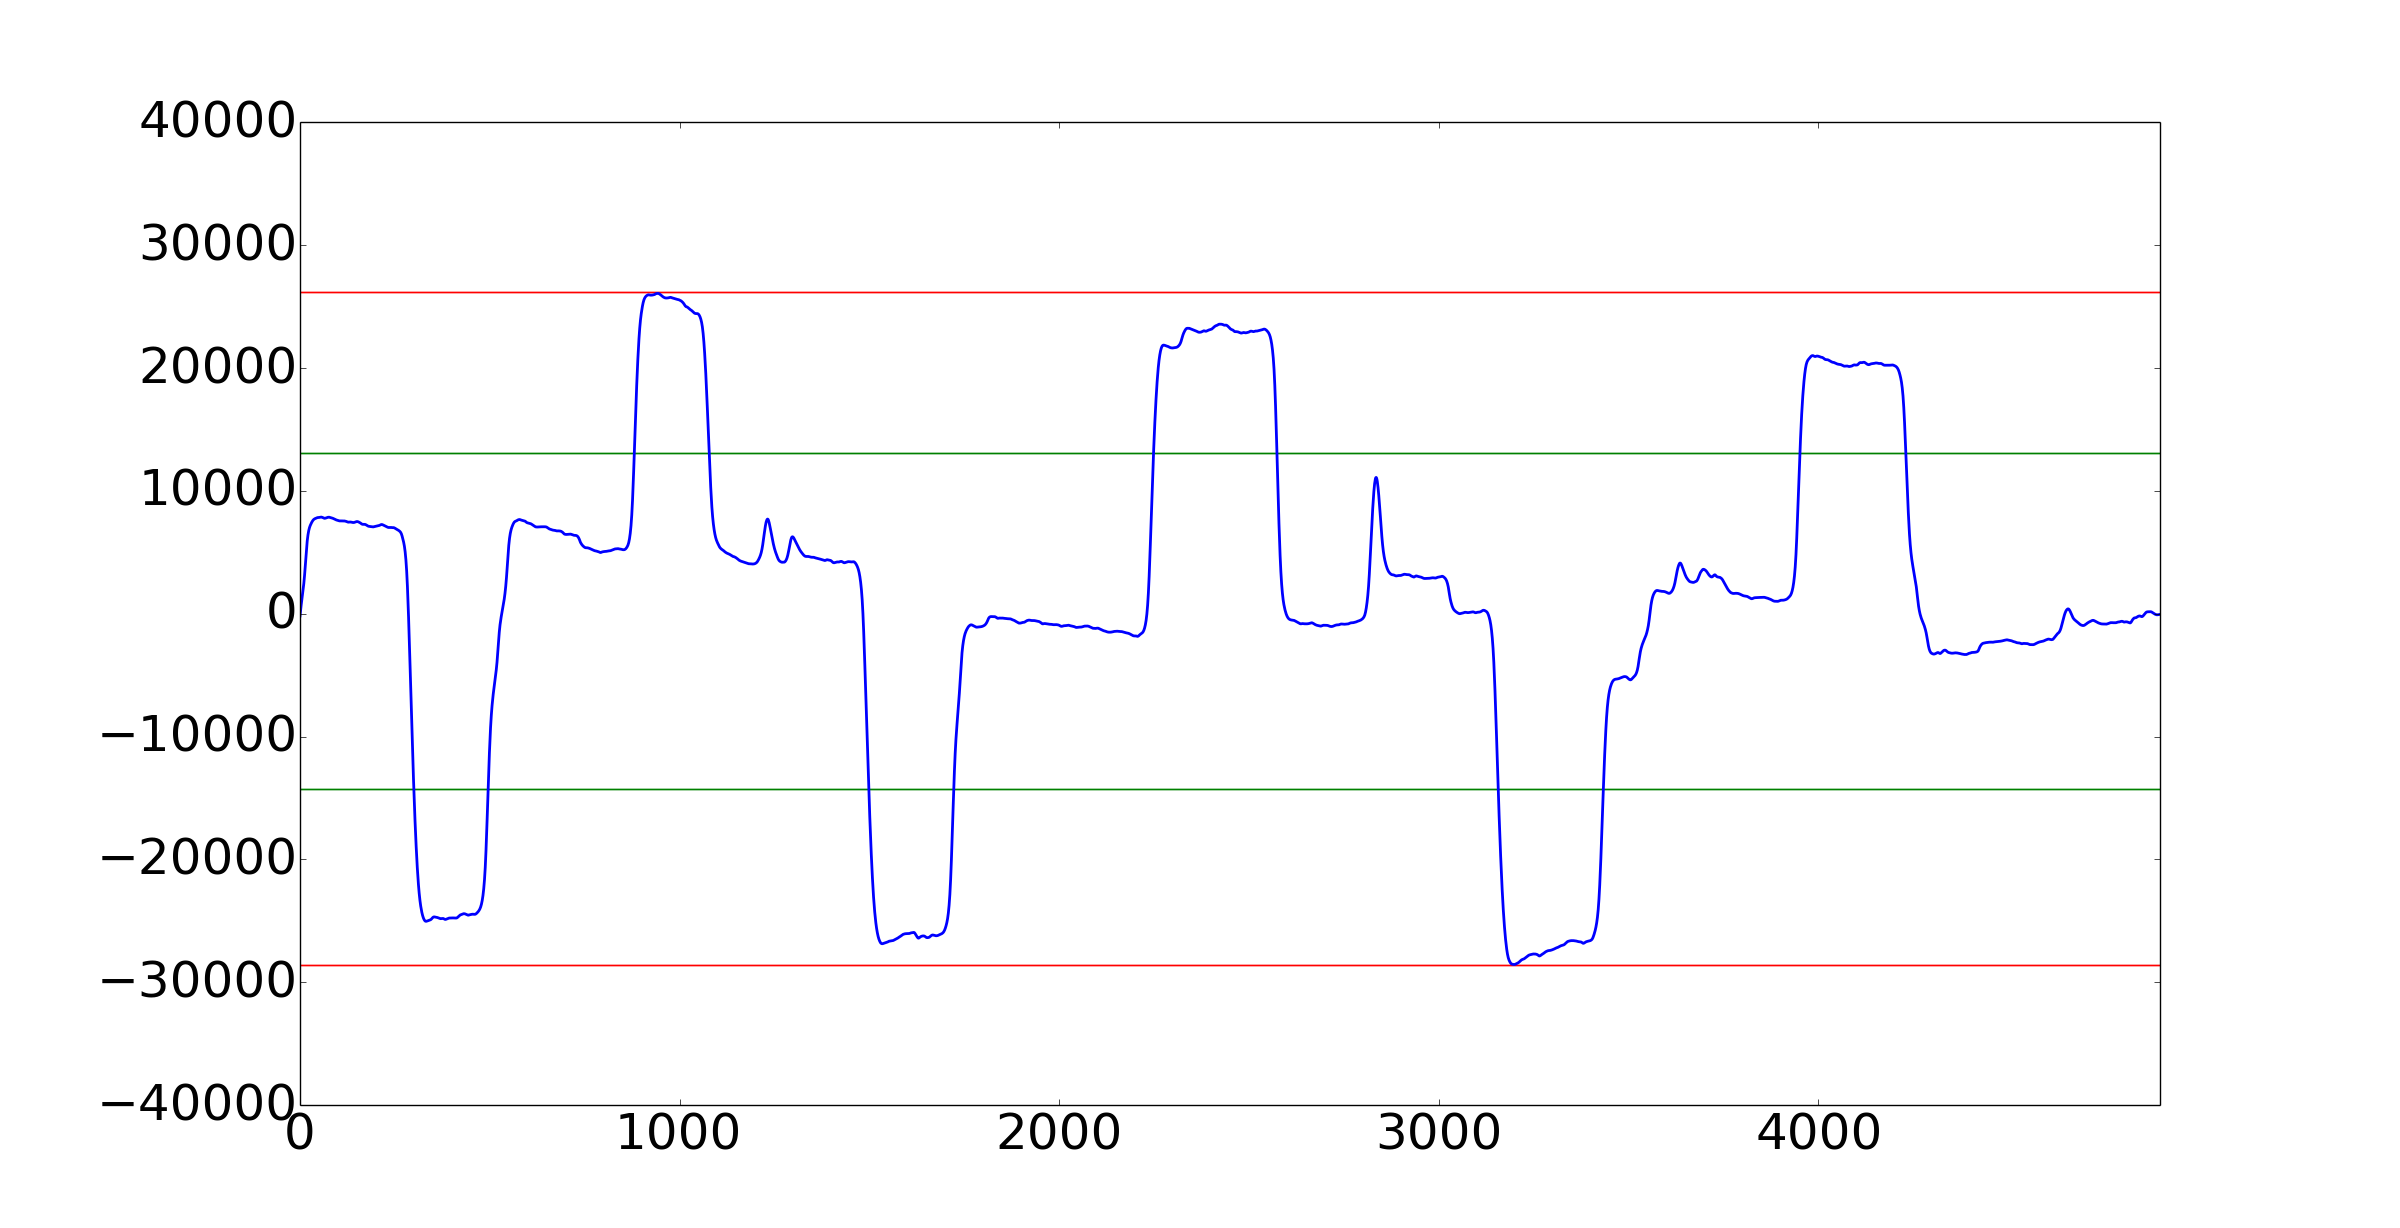
\includegraphics[width=\linewidth]{images/thresholds_distribution}
\caption{In deze afbeelding stellen de rode lijnen het minimum en maximum voor. De groene lijnen zijn het minimum en maximum vermenigvuldigd met $\alpha$.}
\label{fig:maxminthresholds}
\end{figure}

Nu we de bovengrenzen hebben gevonden, moeten we kijkrichtingen gaan zoeken in de nieuwe data. We vragen telkens de 10 recentste datapunten op van de buffer. Om de invloed van een enkele uitschieter in de data te beperken, nemen we telkens het gemiddelde van deze 10 punten. Dit gemiddelde gaan we dan vergelijken met alle bovengrenzen. Slechts wanneer de grenzen 3 opeenvolgende keren overschreden worden, zullen we beslissen dat er een kijkrichting is gevonden.

Omdat we telkens opnieuw de preprocessing-fase uitvoeren op de bufferdata, moeten we oppassen voor het probleem bij veelvuldige herhaling van dezelfde kijkrichting. Zoals eerder vermeld in de thresholds-sectie van gebruikte methoden, zorgt dit voor een verschuiving van het signaal ten opzichte van de y-as. Aangezien we in de herkennings-fase weinig controle hebben over de volgorde van kijkrichtingen, zullen we dit probleem op een andere manier moeten oplossen. Hiervoor gebruiken we afvlakking van het signaal. Telkens als er een threshold overschreden wordt, gaan we het gemiddelde van de vorige 490 datapunten berekenen. Vervolgens vervangen we de originele grensoverschrijdende waardes door dit gemiddelde. Door deze afvlakking, zal de benadering van de biopotentiaal eerder stabiel zijn. Het nadeel van deze techniek is dat de data destructief wordt aangepast en zo mogelijk data verloren gaat. Dit heeft echter geen invloed op dit systeem, aangezien we enkel geïnteresseerd zijn in de nieuwste data. In de figuren~\ref{fig:afvlakking_original} en~\ref{fig:afvlakking} is te zien hoe het signaal veranderd onder afvlakking.

\begin{figure}[h]
\centering
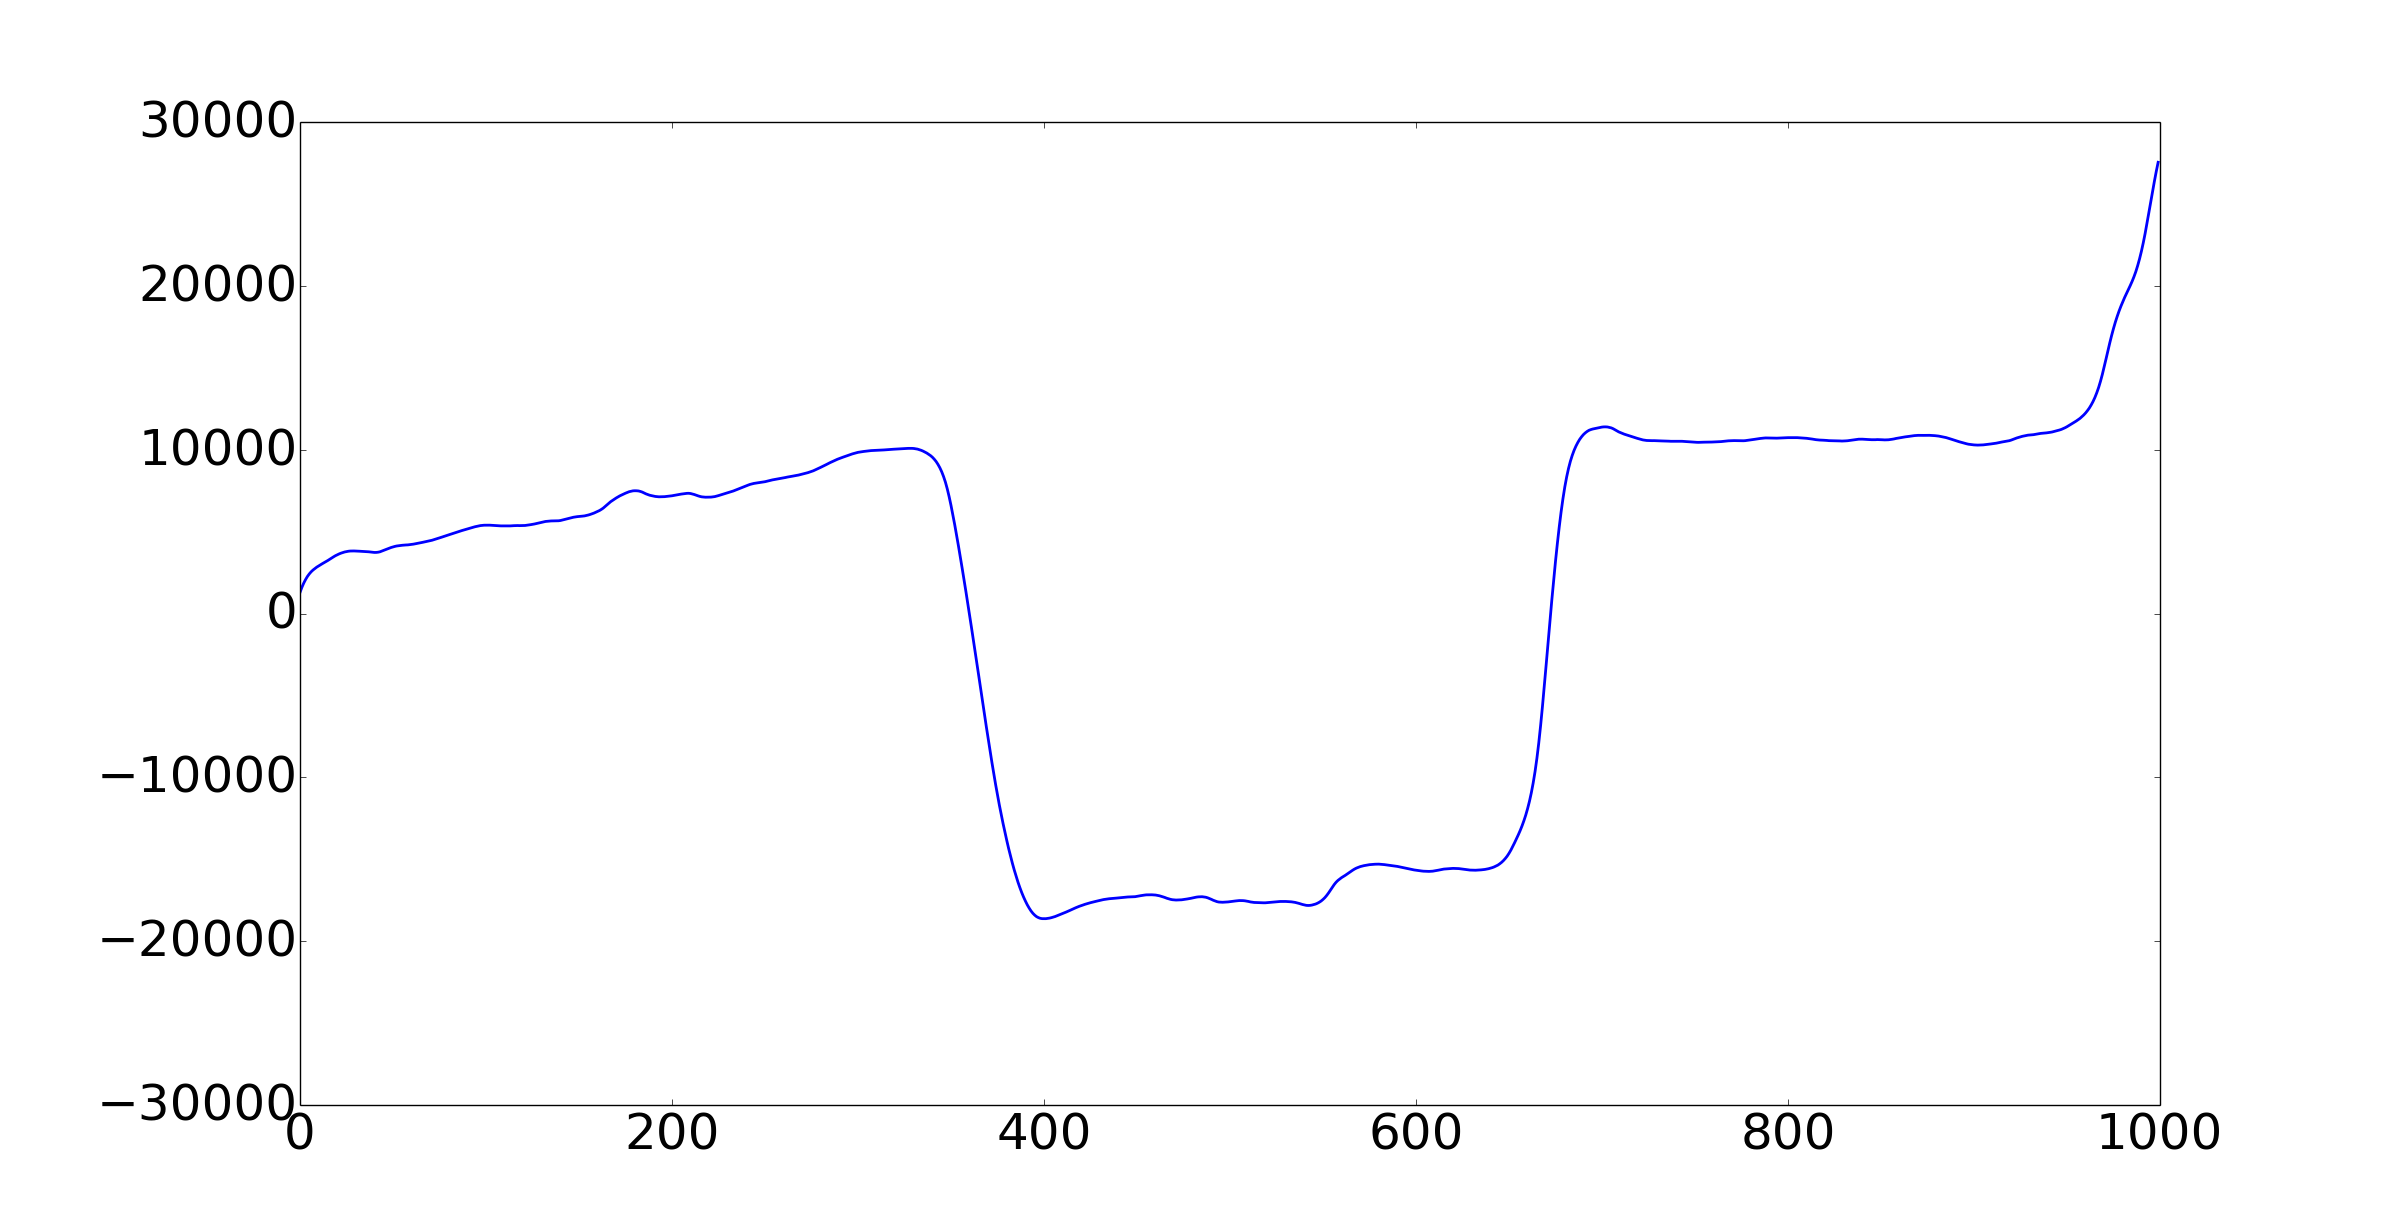
\includegraphics[width=\linewidth]{images/afvlakking_original}
\caption{Dit is een voorbeeld van een gefilterd signaal waarbij geen afvlakking op uitgevoerd is.}
\label{fig:afvlakking_original}
\end{figure}

\begin{figure}[h]
\centering
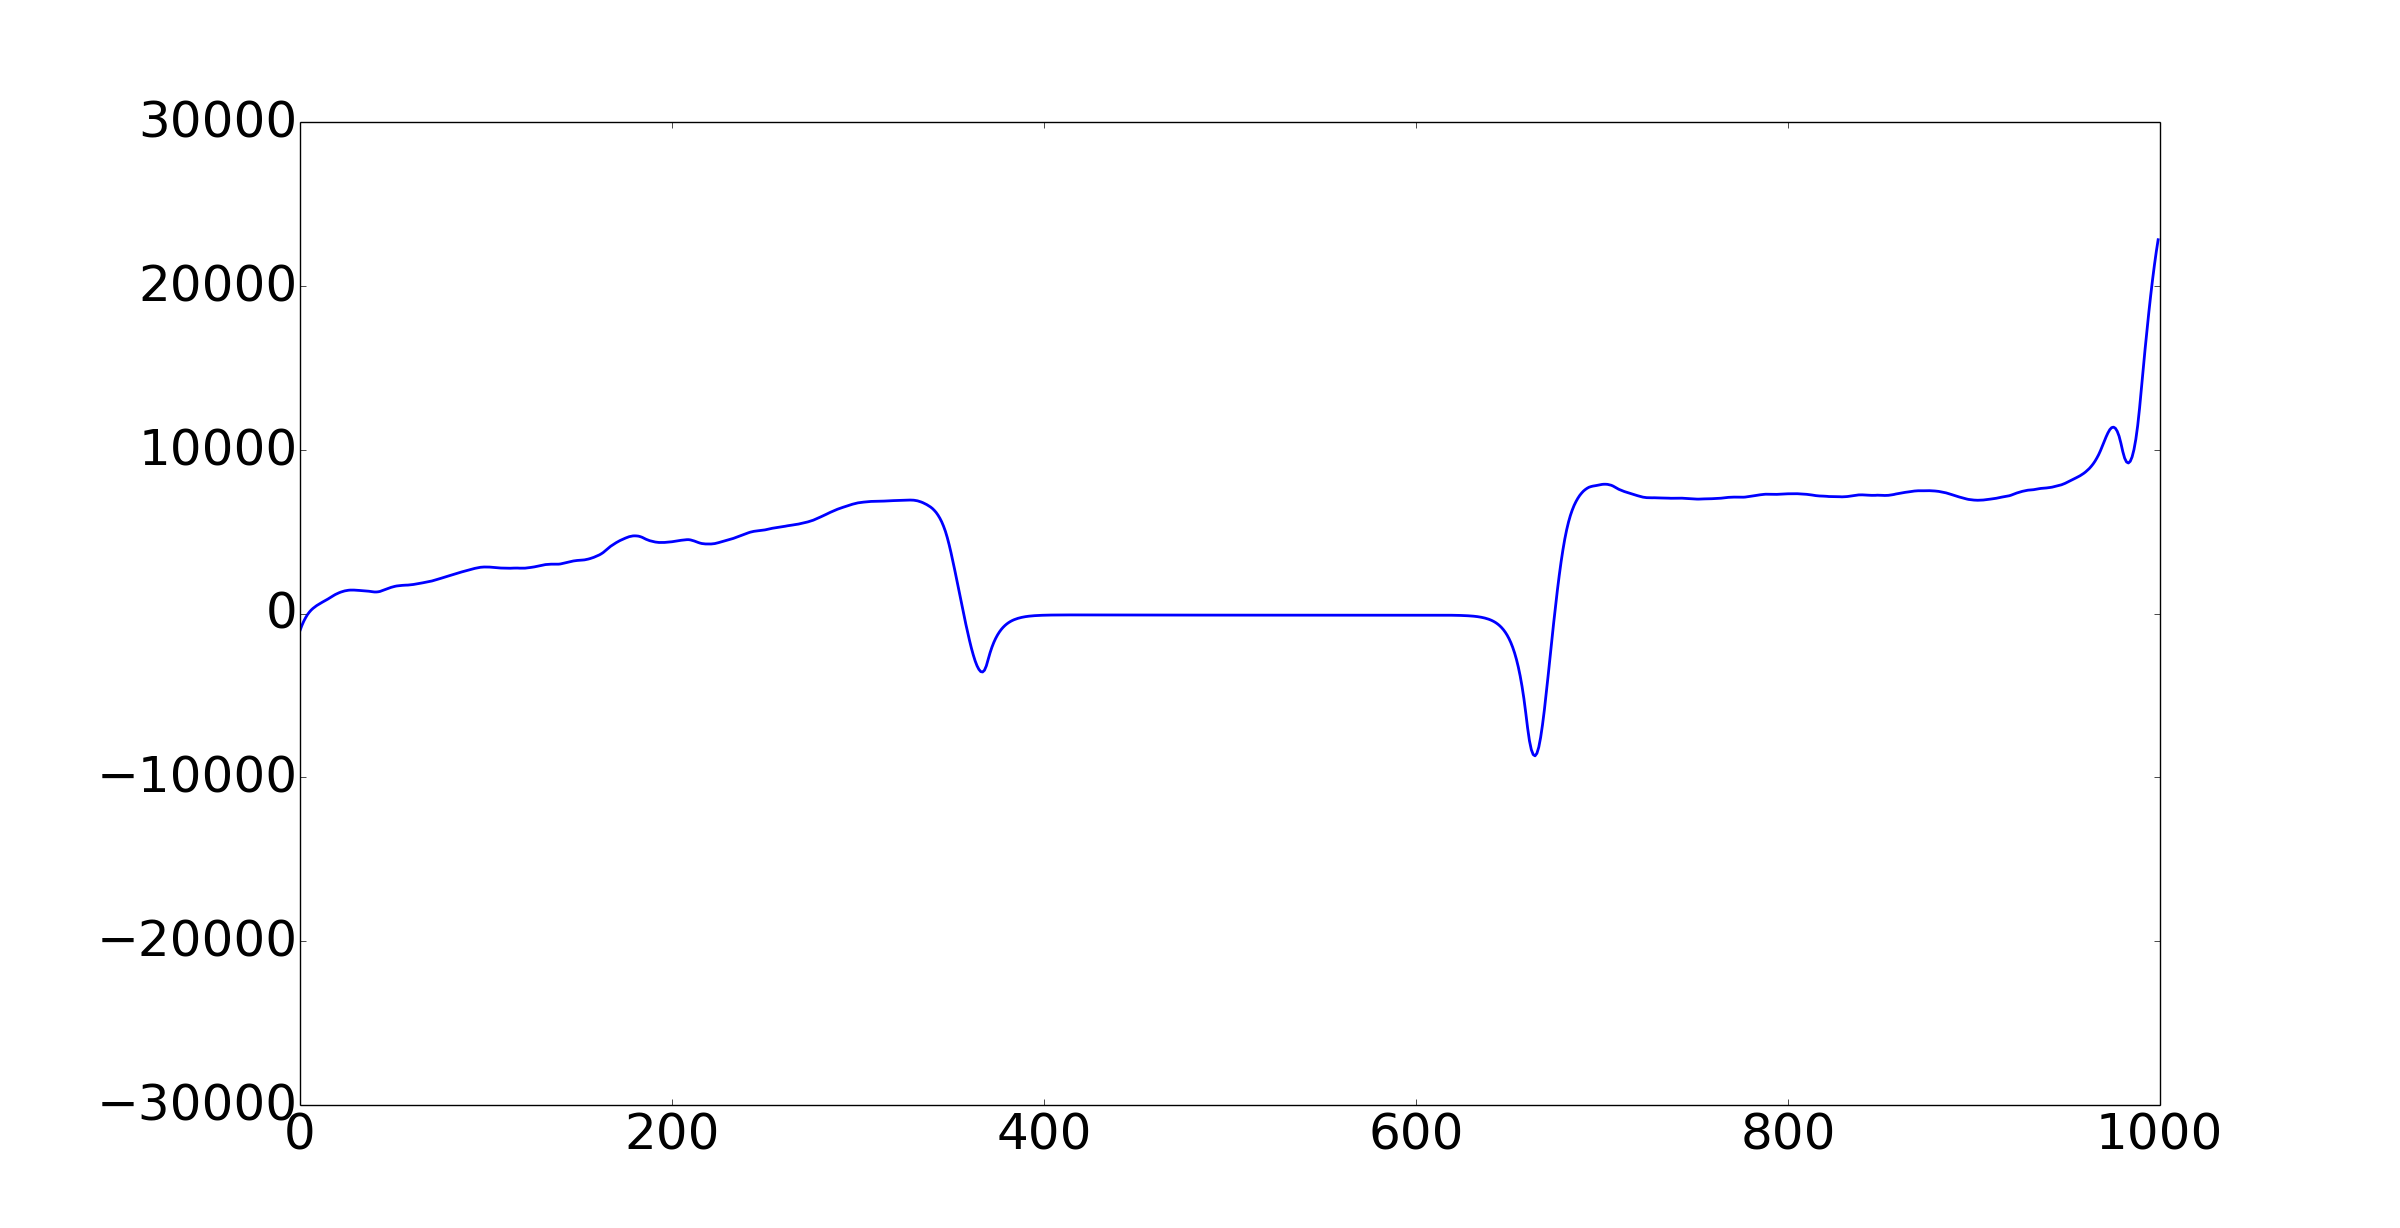
\includegraphics[width=\linewidth]{images/afvlakking}
\caption{Dit is hetzelfde gefilterde signaal uit figuur~\ref{fig:afvlakking_original} waarbij wel een afvlakking op is uitgevoerd. De waarden in deze grafiek zijn nu minder extreem en liggen dichter bij 0.}
\label{fig:afvlakking}
\end{figure}

\subsection{Patronen}

In de calibratie-fase beschikken we over verschillende datasets die gelinkt zijn aan een bepaalde kijkrichting. Voor elke kijkrichting zoeken we minstens één paar van motieven. Deze motieven noemen we het beginmotief en het eindmotief. Een voorbeeld hiervan is te zien in figuur~\ref{fig:beginend}. Deze motieven nemen elk een deel van de hele kijkrichting voor hun rekening. Om telkens zo een paar te verkrijgen, leggen we een aantal voorwaarden op. Zo mogen de motieven elkaar nooit overlappen en moet elk hiervan een verschil in hoogte bestrijken. Dit laatste zorgt ervoor dat we nooit quasi horizontale lijnen, die weinig informatie bevatten, als motief zullen vinden.

\begin{figure}[h]
\centering
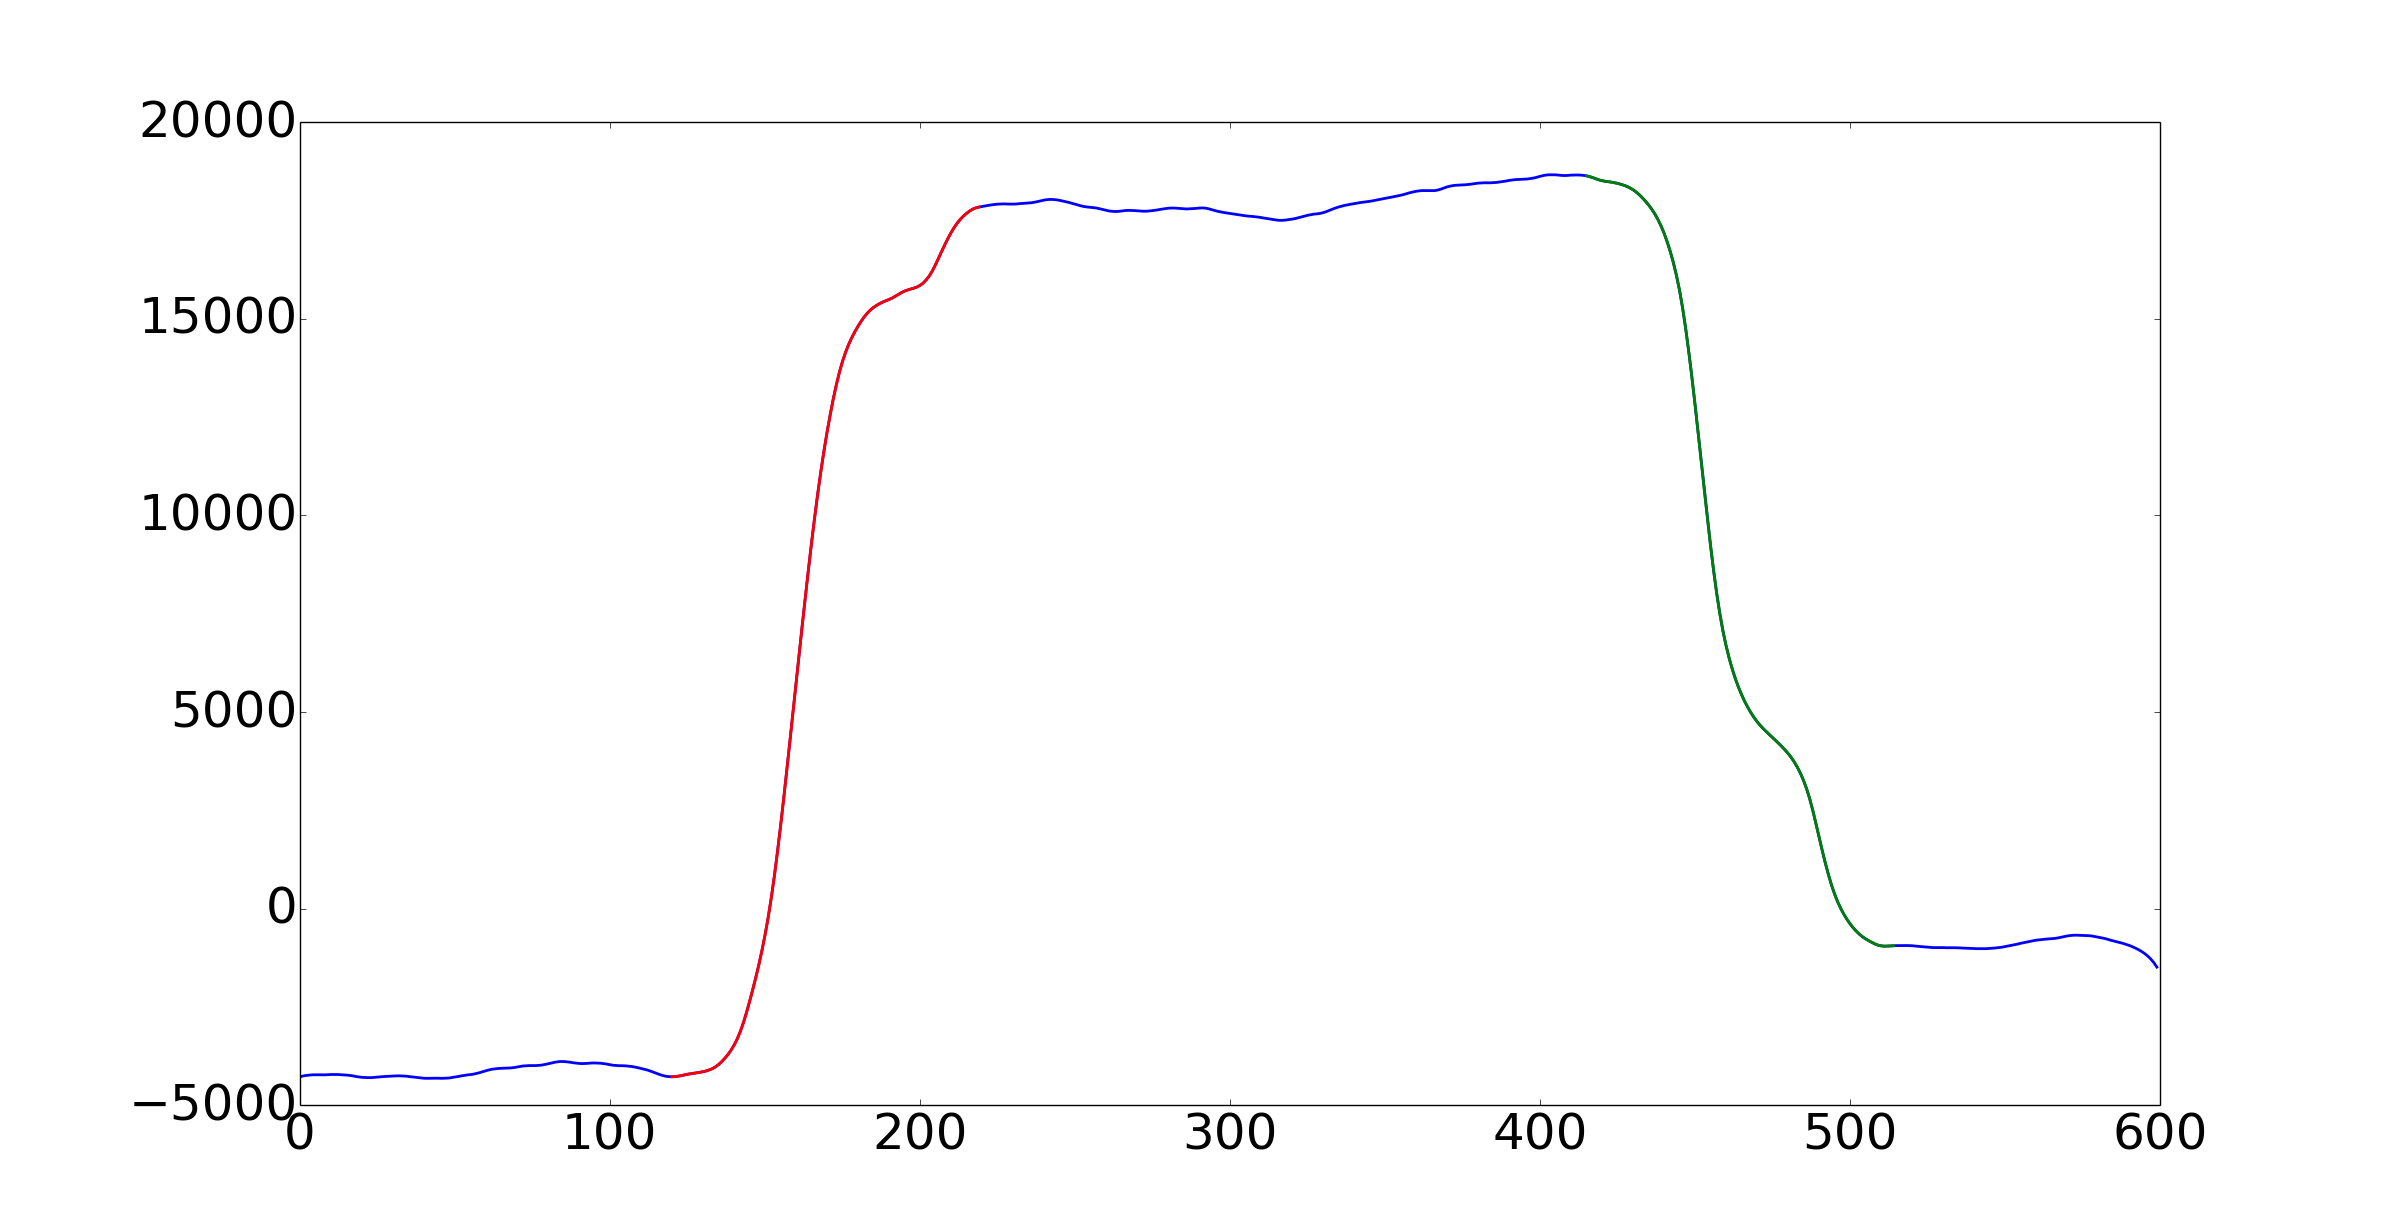
\includegraphics[width=\linewidth]{images/motif_begin_end}
\caption{In deze dataset is het beginmotief aangeduid in het rood en is het eindmotief aangeduid in het groen.}
\label{fig:beginend}
\end{figure}

Voordat we de echte sequenties met elkaar gaan vergelijken, doen we dit eerst met hun genormaliseerde SAX-woorden. Zo kunnen we, zonder al te veel berekeningen, achterhalen welke sequenties in aanmerking komen voor een match. Hiervoor gebruiken we 10 maskers die we op voorhand hebben gedefinieerd. Bij het handmatig opstellen van de maskers, hebben we geprobeerd elke letter even belangrijk te maken, door elke letter even vaak zichtbaar te houden. Een voorbeeld voor een masker is [1,1,0,0], het laat enkel de eerste twee letters zichtbaar.  Zo een masker dekt telkens enkele letters van twee te vergelijken SAX-woorden af, zie voorbeelden in \ref{seq:maskering}. 

\begin{equation}
\label{seq:maskering}
\begin{aligned}
abcd \times [1,1,0,0] = ab \\
abcd \times [0,1,1,0] = bc \\
abcd \times [1,0,0,1] = ad \\
\end{aligned} 
\end{equation}

Deze maskers gebruiken we bij het opstellen van de collision matrix. Elke cel in deze matrix hoort bij een paar van sequenties. De waarde in een cel geeft weer hoe goed de bijhorende sequenties op elkaar lijken. We beginnen met een lege collision matrix. Eerst nemen we het eerste masker en dekken er de SAX-woorden van alle sequenties mee af. Dan kijken we naar elk paar sequenties en indien de gemaskeerde woorden hetzelfde zijn, incrementeren we de waarde in de bijhorende cel. Dit herhalen we voor elk masker. Daarna kijken we naar de waarden uit de gevulde collision matrix. Voor elke cel met een waarde groter dan of gelijk aan de collision threshold komt het bijhorende paar in aanmerking als match. Elk paar sequenties dat in aanmerking komt om een match te zijn, wordt dan eindelijk echt vergeleken. Dit gebeurt door de euclidische afstand tussen de genormaliseerde sequenties te berekenen. Pas als deze afstand kleiner is dan een vooraf gedefinieerde variabele $range$, spreken we van een match.

\begin{table}
\caption{Dit is een voorbeeld van een complete collision matrix. De vier SAX-woorden van verschillende sequenties staan bij een kolom en rij. De matrix is maar half ingevuld omdat hij symmetrisch is.  De diagonaal is leeg, omdat sequenties niet met zichzelf worden vergeleken. De gebruikte maskers staan onder de tabel.}
\label{tab:collision_matrix}
\centering
\begin{tabular}{ l || c | c | c | c }
& accd & dcda & acda & acda \\ \hline
\hline
accd & / & 0 & 1 & 1 \\ \hline
dcda & / & / & 2 & 2 \\ \hline
acda & / & / & / & 4 \\ \hline
acda & / & / & / & / \\
\hline
\end{tabular}\par

$[1,1,0,0], [0,0,1,1], [1,0,0,1], [0,1,1,0]$
\end{table}

Tijdens de calibratie, vergroten we de collision matrix dynamisch. Dit doen we zodat na de calibratie-fase, niet alle data in één keer verwerkt moet worden, maar wel al tussen door kan gebeuren. Bij de eerste twee sequenties die worden toegevoegd, wordt nog gewoon een collision matrix opgesteld. Bij de derde en volgende sequenties, wordt er een nieuwe rij en kolom toegevoegd die overeenkomt met de nieuwe sequentie. Hiervoor worden de benodigde cellen berekend en ingevuld. [TODO]

Nu we alle matches hebben gevonden, kunnen we elke sequentie aan een lijst met al zijn matches koppelen. Met behulp van deze lijsten, kunnen we de sequenties rangschikken. We sorteren alle sequenties op het aantal matches dat ze hebben, met de sequentie met de meeste matches vooraan. In het geval dat twee sequenties evenveel matches zouden hebben, krijgt de sequentie met de kleinste totale euclidische afstand tot zijn matches voorrang.

In de herkennings-fase worden, na elke nieuwe toevoeging van tien datapunten, de laatste honderd datapunten opgevraagd. Deze honderd datapunten vormen een sequentie. Net zoals in de calibratie, wordt ook voor deze sequenties gecontroleerd of ze wel een groot genoeg hoogteverschil hebben. De sequentie wordt genormaliseerd en gediscretiseerd naar een SAX-woord. Met behulp van de eerder gebruikte maskers wordt nu ook nagegaan of de sequentie goed genoeg lijkt op een motief. Telkens beide gemaskeerde SAX-woorden gelijk zijn, spreken we van een collision. Indien het aantal collisions groter is dan de collision threshold, worden de sequenties zelf weer vergeleken. Dit gebeurt ook hier met behulp van de euclidische afstand. Indien de afstand voldoet aan de eerder vermeldde $range$, wordt het label van het motief gegeven aan deze sequentie. Dit betekent dat we het motief hebben herkend. 

Pas wanneer achtereenvolgens het beginmotief en het eindmotief herkend worden, gaan we uit van een kijkrichting. Indien het beginmotief herkend wordt en de herkenning van het eindmotief op zich laat wachten, zal een timer ervoor zorgen dat er niet oneindig lang gewacht wordt op de herkenning van het eindmotief.


\section{Experimenten}

Bij het uitvoeren van experimenten hebben we ons vooral geconcentreerd op de thresholds-methode. Aangezien de patronen-methode zoveel afhangt van verschillende parameters, hebben we dit nog niet kunnen optimaliseren. Hierom hebben we op deze methode geen experimenten uitgevoerd, zodat we geen vertekend beeld zouden scheppen over de mogelijkheden van de patronen.

De opstelling van de experimenten zag er als volgt uit. De sensoren zijn bevestigd op de het gezicht van de gebruiker door middel van stevige plakkers. Deze moeten blijven plakken zonder tussenkomst van de handen. De sensoren die verantwoordelijk zijn voor het meten van de kijkrichtingen links en rechts zijn bevestigd op de slapen, tegen de ooghoeken. De sensoren verantwoordelijk voor de kijkrichtingen boven en onder hebben we niet gebruikt in deze experimenten. De gebruiker zit op een stoel en kijkt voor zich uit. Hierbij is het ook belangrijk dat de gebruiker niet afgeleid kan worden door bewegende voorwerpen. Het gebruiken van andere gezichtsspieren dan de oogspieren moet zo veel mogelijk vermeden worden. De sensoren vangen de signalen van deze spieren namelijk ook op. Lachen kan bijvoorbeeld niet, rustig praten kan zolang het niet zichtbaar is in het gemeten signaal.

De sensoren zijn aangesloten op een EOG Bord, gemaakt door InnovationLab van de KU Leuven. Dit apparaat voert al een redelijk naïve biopotentiaalfiltering uit op het signaal. Het vlakt het signaal altijd af naar de neutrale waarde (de waarde verkregen bij het rechtdoor kijken). Hierdoor wordt de intensiteit van het kijken naar links en rechts geleidelijk aan afgezwakt.

We concentreren ons in deze experimenten op de events die gebeuren. Het kijken naar links is bijvoorbeeld een event. Dit doen we omdat we meer geïnteresseerd zijn in detecteren van deze events, dan TODO.We duiden reeksen van kijkrichtingen aan volgens de definitie van reeks~\ref{seq:definitie}. We bepalen drie verschillende kijkrichtigen elk met een tijd. Deze tijd $t_i$ staat voor het aantal seconden dat ongeveer in de bijhorende kijkrichting gekeken wordt. $h$ geeft aan hoeveel keer de reeks binnen de accolades herhaald wordt.

\begin{equation}
\label{seq:definitie}
\begin{aligned}
& rechtdoor(t_1),  links (t_1), rechts (t_2) \\
& \{ A, B\} \times h = A_1, B_1, A_2, B_2, ... , A_h, B_h
\end{aligned}
\end{equation}

In de calibratie-fase werd er telkens volgens reeks~\ref{seq:calibratie} gekeken.

\begin{equation}
\label{seq:calibratie}
\begin{aligned}
&\{rechtdoor(1), links(1), &\\
&rechtdoor(1), rechts(1)\} \times 2, &\\
& rechtdoor(1)&
\end{aligned}
\end{equation}

Resultaten verwerken we door middel van een confusion matrix. Elke rij en kolom stelt een kijkrichting voor. Aan de hand van deze matrix berekenen we de $accuracy$ (\ref{eq:accuracy}), $recall_k$ (\ref{eq:recall}) en $precision_k$ (\ref{eq:precision}). Hierbij staat $k$ voor de relevante kijkrichting. $accuracy$ staat voor de verhouding tussen de correct herkende kijkrichtingen en alle te herkennen kijkrichtingen. $recall_k$ staat voor de verhouding tussen de correct herkende kijkrichtingen $k$ en alle werkelijk gekeken kijkrichtingen $k$. $precision_k$ staat voor de verhouding tussen correct herkende kijkrichtingen $k$ en alle herkende kijkrichtingen $k$. De kijkrichting $rechtdoor$ geven we een zeer klein gewicht van $1/10$ mee, omdat deze kijkrichting veel gebruikt wordt in de experimenten en een vertekend beeld kan scheppen.

\begin{table}[h]
\caption{Deze tabel stelt de confusion matrix voor. Als de gebruiker bijvoorbeeld naar $links$ kijkt, maar we detecteren de kijkrichting $rechts$, zal de cel d met 1 verhoogd worden. Op de diagonaal (de cellen a, e en i) staan alle succesvolle voorspellingen.}
\centering
\begin{tabular}{ l || c | c | c }
\backslashbox{Herkend~}{Echt~~}
& $links$ & $rechts$ & $rechtdoor$ \\ \hline
\hline
$links$ & a & b & c \\ \hline
$rechts$ & d & e & f \\ \hline
$rechtdoor$ & g & h & i \\
\hline
\end{tabular}\par
\end{table}

\begin{equation}
\label{eq:accuracy}
accuracy = \frac{a + e + \frac{i}{10}}{a + b + c + d + e + f + g + h + \frac{i}{10}}
\end{equation}

\begin{equation}
\begin{aligned}
\label{eq:recall}
recall_{links} = \frac{a}{a + d + g} \\
recall_{rechts} = \frac{e}{b + e + h}
\end{aligned}
\end{equation}

\begin{equation}
\begin{aligned}
\label{eq:precision}
precision_{links} = \frac{a}{a + b + c} \\
precision_{rechts} = \frac{e}{d + e + f}
\end{aligned}
\end{equation}

Deze testen zijn uitgevoerd op twee verschillende personen. We noemen ze \textit{gebruiker 1} en \textit{gebruiker 2}. We laten de gebruikers elke reeks vijf keer uitvoeren, om zo een betrouwbaar beeld te krijgen van de prestaties van het programma.

\subsection{Experiment 1}

In dit experiment laten we een gebruiker reeks~\ref{seq:exp1} volgen. Figuur~\ref{fig:exp1} toont een voorbeeld van hoe het signaal er uitziet voor deze reeks. 

\begin{equation}
\begin{aligned}
\label{seq:exp1}
& \{rechtdoor(5), links(2)\} \times 5,& \\
& \{rechtdoor(5), rechts(2)\} \times 5,& \\
& rechtdoor(5) &
\end{aligned}
\end{equation}

De gebruiker moet volgens reeks~\ref{seq:exp1} afwisselend links en rechts kijken. We gebruiken eerst deze volgorde, omdat deze zoals eerder vermeld geen problemen oplevert tijdens de preprocessing-stap. We willen eerst weten hoe goed het systeem werkt in ideale omstandigheden, voordat we de minder ideale situaties bekijken. Deze resultaten hebben we in een confusion matrix, tabel~\ref{tab:exp1} en~\ref{tab:exp1_2}, weergegeven.


\begin{figure}[h]
\centering
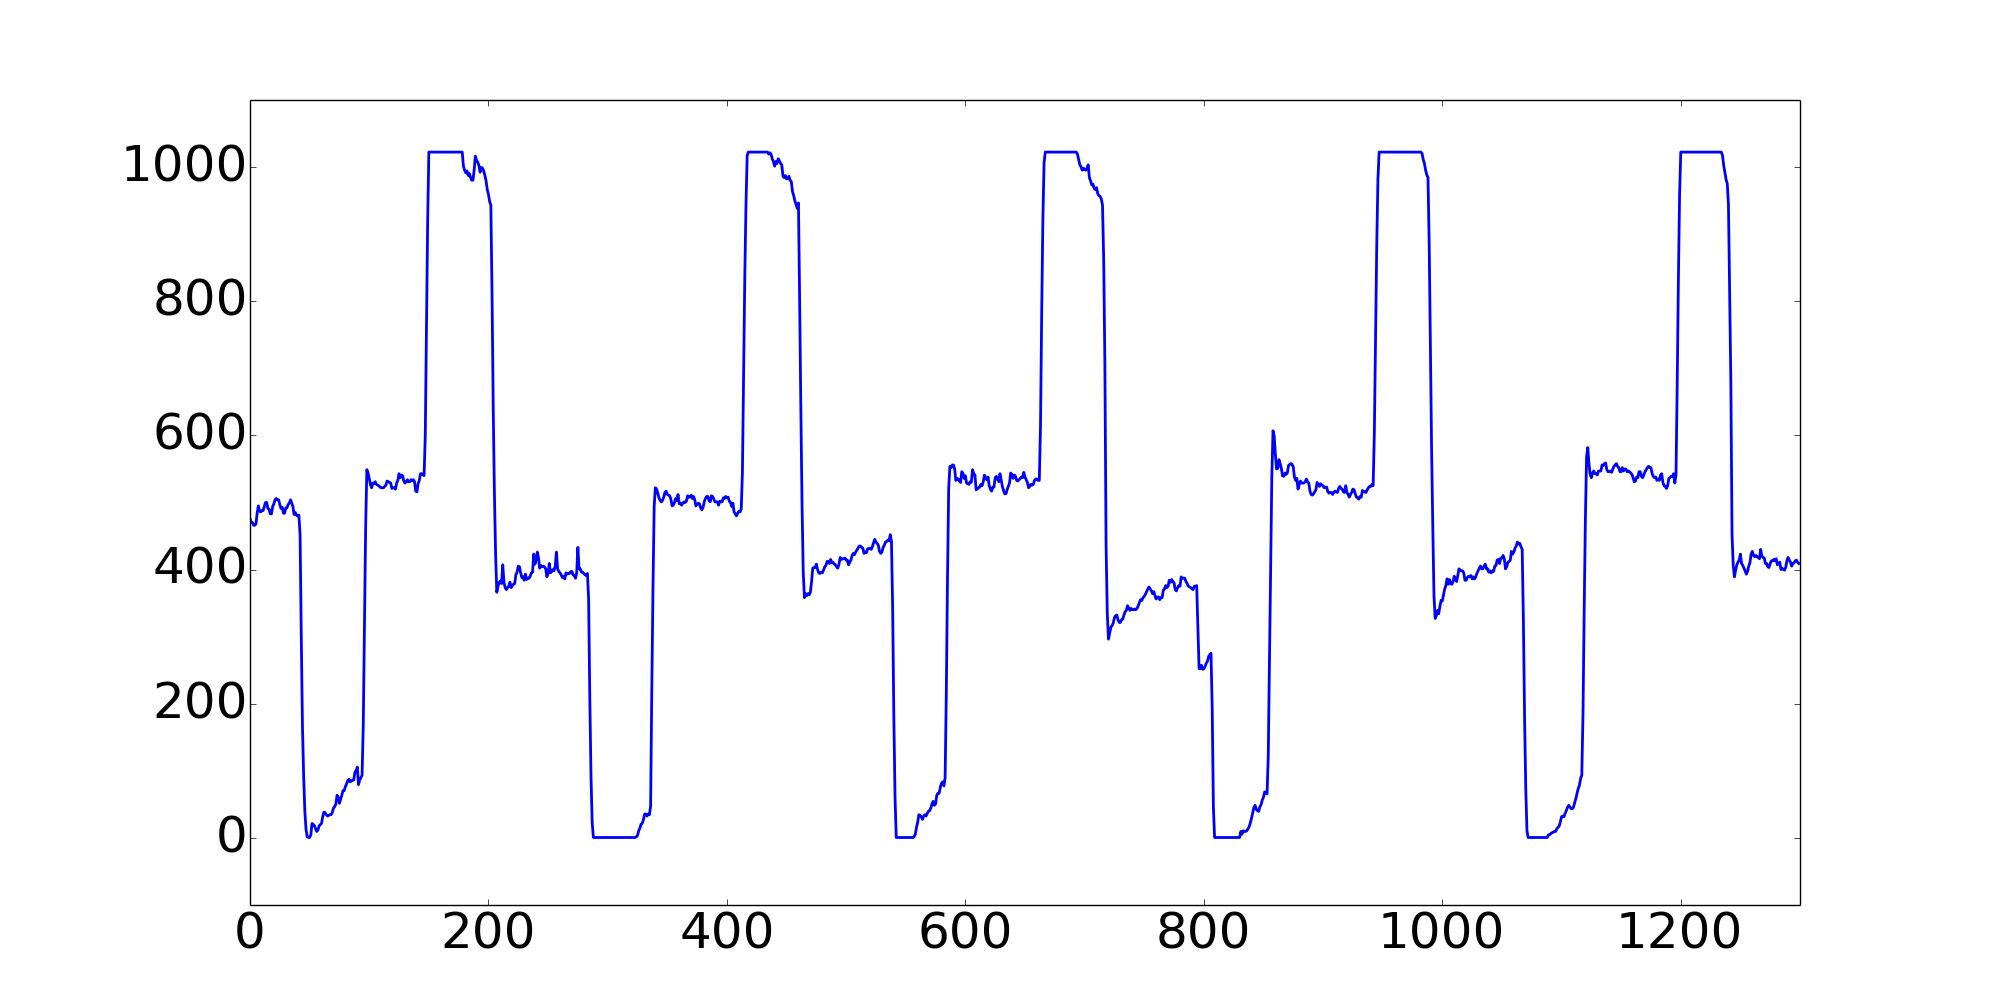
\includegraphics[width=\linewidth]{images/experiment1}
\caption{Een voorbeeld signaal bij uitvoering van experiment 1. Er is duidelijk te zien dat er telkens van kijkrichting gewisseld wordt.}
\label{fig:exp1}
\end{figure}

\begin{table}[h]
\caption{Confusion matrix na uitvoering van experiment 1 door \textit{gebruiker 1} en de berekende maatstaven.}
\label{tab:exp1}
\centering
\begin{tabular}{ l || c | c | c }
\backslashbox{Herkend~}{Echt~~}
& $links$ & $rechts$ & $rechtdoor$ \\ \hline
\hline
$links$ & 18 & 0 & 0 \\ \hline
$rechts$ & 0 & 25 & 0 \\ \hline
$rechtdoor$ & 7 & 0 & 55 \\
\hline
\end{tabular}\par

\begin{equation*}
\begin{aligned}
&accuracy = 0,87 &\\
& precision_{links} = 1 & recall_{links} = 0,72 & \\
& precision_{rechts} = 1 & recall_{rechts} = 1 &
\end{aligned}
\end{equation*}

\end{table}


We kunnen uit deze resultaten enkele conclusies trekken. De precision van beide kijkrichtingen, links en rechts, zijn 1. Dit geldt bij beide gebruikers. Hierdoor weten we dat het systeem nooit incorrect links of rechts herkend heeft. Bij de recall merken we wel dat er voor \textit{gebruiker 1} problemen waren bij het herkennen van van links. Voor \textit{gebruiker 2} waren er echter vooral problemen bij het herkennen van links. Hieruit kunnen we afleiden dat een kleine verandering in omstandigheden een verschil maakt voor de recall, maar niet voor de precision. Adnerzijds merken we op dat er geen fouten zijn gebeurt telkens er rechtdoor werd gekeken. De recall voor rechtdoor is bjgevolg 1. Ook zien we dat beide gebruikers toevallig exact dezelfde accuracy hebben. Deze accuracy van 0.87 is al vrij goed, maar betekent wel dat er nog veel verbetering mogelijk is. 

\begin{table}[h]
\caption{Confusion matrix na uitvoering van experiment 1 door \textit{gebruiker 2} en de berekende maatstaven.}
\label{tab:exp1_2}
\centering
\begin{tabular}{ l || c | c | c }
\backslashbox{Herkend~}{Echt~~}
& $links$ & $rechts$ & $rechtdoor$ \\ \hline
\hline
$links$ & 24 & 0 & 0 \\ \hline
$rechts$ & 0 & 19 & 0 \\ \hline
$rechtdoor$ & 1 & 6 & 55 \\
\hline
\end{tabular}\par

\begin{equation*}
\begin{aligned}
&accuracy = 0,87 &\\
& precision_{links} = 1 & recall_{links} = 0,96 & \\
& precision_{rechts} = 1 & recall_{rechts} = 0,76 &
\end{aligned}
\end{equation*}

\end{table}



\subsection{Experiment 2}

Nu we weten hoe goed thresholds werken in de ideale omstandigheden, gaan we in het tweede experiment een minder ideale situatie bekijken. We laten de gebruiker meerdere opeenvolgende keren naar dezelfde richting kijken, volgens reeks~\ref{seq:exp2}. Figuur~\ref{fig:exp2} geeft een voorbeeld van hoe het signaal er uit ziet. Zoals we in bij preprocessing hebben vermeld, zal deze volgorde voor problemen kunnen zorgen in de preprocessing-stap. Dit experiment hebben we dan ook gekozen om onze oplossing, afvlakking, uit te testen.

\begin{equation}
\begin{aligned}
\label{seq:exp2}
& \{rechtdoor(5), links(2) & \\
& rechtdoor(5), rechts(2)\} \times 5,& \\
& rechtdoor(5) &
\end{aligned}
\end{equation}


\begin{figure}[h]
\centering
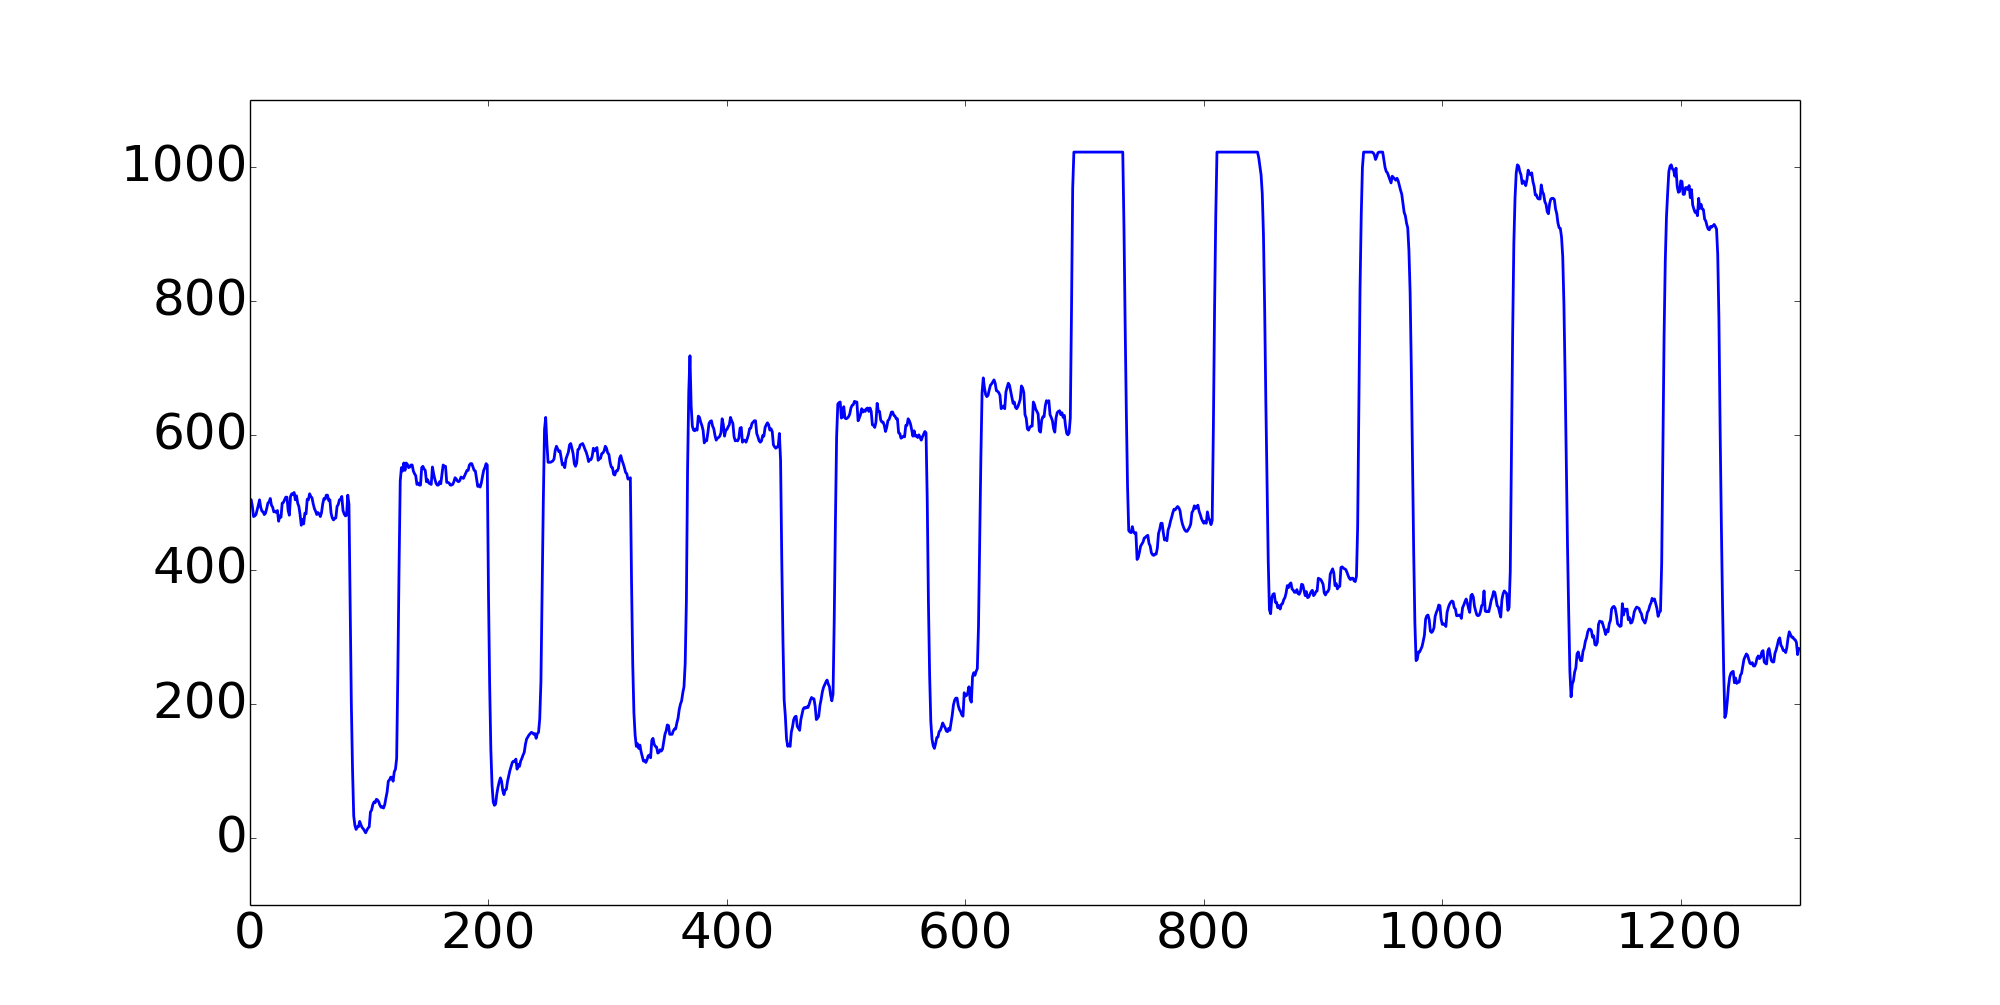
\includegraphics[width=\linewidth]{images/experiment2}
\caption{Een voorbeeld signaal bij uitvoering van experiment 2. Er is duidelijk te zien dat er eerst naar links werd gekeken en daarna naar rechts. Door de naïve biopotentiaalfiltering van de hardware heeft er een verschuiving van waarden plaats gevonden in het signaal. Dit zorgt ervoor dat de bovengrens moeilijker te overschrijden is naarmate men een bepaalde kijkrichting herhaalt.}
\label{fig:exp2}
\end{figure}

\begin{table}[h]
\caption{Confusion matrix na uitvoering van experiment 2 door \textit{gebruiker 1} en de berekende maatstaven.}
\label{tab:exp2}
\centering
\begin{tabular}{ l || c | c | c }
\backslashbox{Herkend~}{Echt~~}
& $links$ & $rechts$ & $rechtdoor$ \\ \hline
\hline
$links$ & 16 & 0 & 5 \\ \hline
$rechts$ & 0 & 14 & 0 \\ \hline
$rechtdoor$ & 9 & 11 & 50 \\
\hline
\end{tabular}\par

\begin{equation*}
\begin{aligned}
&accuracy = 0,58 &\\
& precision_{links} = 0,76 & recall_{links} = 0,64 & \\
& precision_{rechts} = 1 & recall_{rechts} = 0,56 &
\end{aligned}
\end{equation*}

\end{table}



\begin{table}[h]
\caption{Confusion matrix na uitvoering van experiment 2 door \textit{gebruiker 2} en de berekende maatstaven.}
\label{tab:exp2_2}
\centering
\begin{tabular}{ l || c | c | c }
\backslashbox{Herkend~}{Echt~~}
& $links$ & $rechts$ & $rechtdoor$ \\ \hline
\hline
$links$ & 17 & 0 & 1 \\ \hline
$rechts$ & 0 & 8 & 0 \\ \hline
$rechtdoor$ & 8 & 17 & 54 \\
\hline
\end{tabular}\par

\begin{equation*}
\begin{aligned}
&accuracy = 0,54 &\\
& precision_{links} = 0,94 & recall_{links} = 0,68 & \\
& precision_{rechts} = 1 & recall_{rechts} = 0,47 &
\end{aligned}
\end{equation*}

\end{table}

Dit experiment heeft veel minder goede resulaten dan het eerste experiment. De $accuracy$ en $recall$ zijn allebei duidelijk slechter. Dit kunnen we verklaren aan de hand van figuur~\ref{fig:exp2}. Er is duidelijk een verschuiving volgens de y-as te zien, maar dit is een gevolg van de biopotentiaalfiltering van de sensoren zelf. Door het geleidelijk afzwakken van het signaal terwijl er naar links of rechts gekeken wordt, zal bij het terug rechtdoor kijken, het signaal niet rond de neutrale lijn liggen. Het zal eerder uitwijken naar de tegenovergestelde kijkrichting, waardoor het moeilijker wordt om herhaalde kijkrichtingen te herkennen. Dit verklaart de lage $recall$ voor beide kijkrichtingen. Hieruit leiden we af dat deze naïve biopotentiaalfiltering niet de beste oplossing is voor alle situaties.

\subsection{Experiment 3}

Het apparaat dat we gebruiken probeert de biopotentiaalschommelingen te filteren door telkens het signaal langzaam af te vlakken naar de neutrale staat (de staat wanneer er rechtdoor gekeken wordt). Wanneer er bijvoorbeeld lang naar links gekeken wordt, verschuift het signaal volgens de y-as. Als er nu terug rechtdoor gekeken wordt, lijkt het alsof er naar rechts gekeken wordt. We verwachtten dat als tussen het links en rechts kijken voor een langere periode rechtdoor gekeken wordt, dit effect teniet wordt gedaan. Dit hebben we getest in dit experiment.

\begin{figure}[h]
\centering
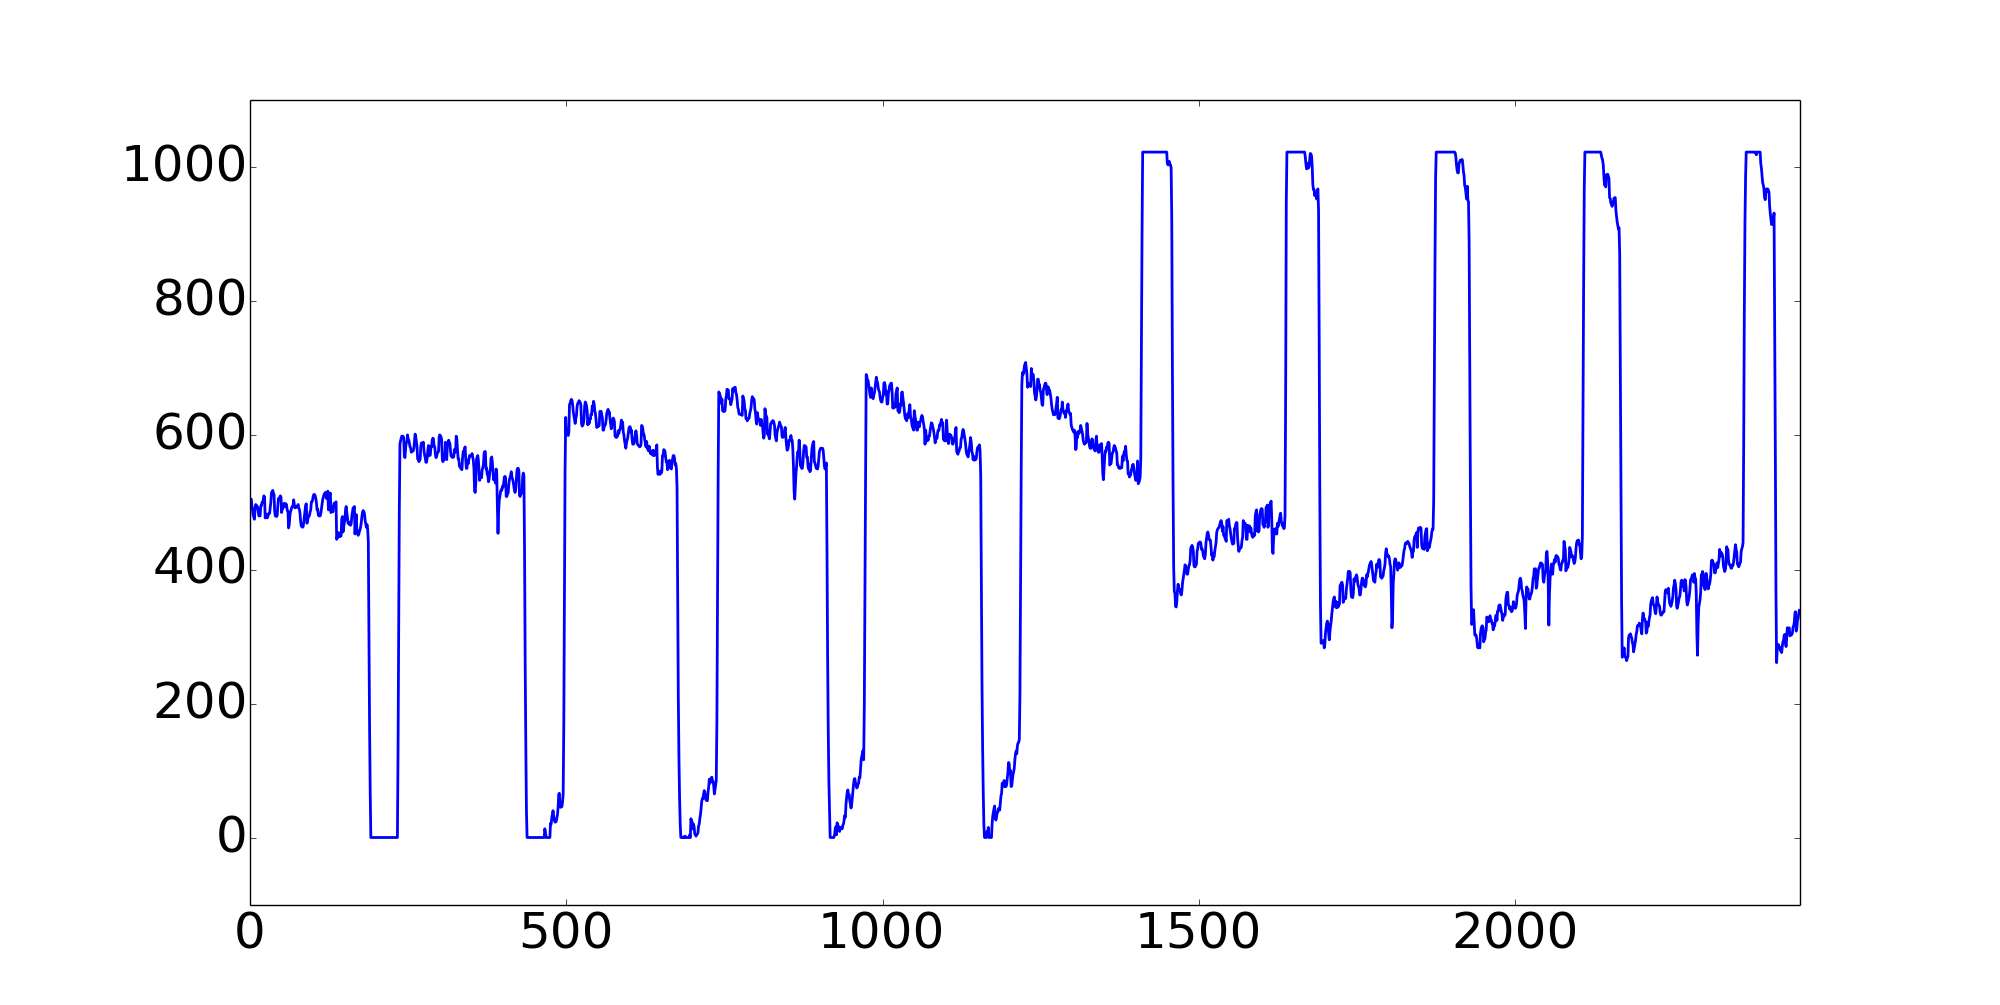
\includegraphics[width=\linewidth]{images/experiment3}
\caption{Een voorbeeld signaal bij uitvoering van experiment 3. We merken op dat door langer rechtdoor te kijken tussen andere kijkrichtingen in, het besproken effect niet meer voorkomt. }
\label{fig:exp3}
\end{figure}

\begin{equation}
\begin{aligned}
\label{seq:exp3}
& \{rechtdoor(10), links(3) & \\
& rechtdoor(10), rechts(3)\} \times 5,& \\
& rechtdoor(10) &
\end{aligned}
\end{equation}

\begin{table}[h]
\caption{Confusion matrix na uitvoering van experiment 3 door \textit{gebruiker 1} en de berekende maatstaven.}
\label{tab:exp3}
\centering
\begin{tabular}{ l || c | c | c }
\backslashbox{Herkend~}{Echt~~}
& $links$ & $rechts$ & $rechtdoor$ \\ \hline
\hline
$links$ & 24 & 0 & 1 \\ \hline
$rechts$ & 0 & 20 & 0 \\ \hline
$rechtdoor$ & 1 & 5 & 54 \\
\hline
\end{tabular}\par

\begin{equation*}
\begin{aligned}
&accuracy = 0,88 &\\
& precision_{links} = 0,96 & recall_{links} = 0,96 & \\
& precision_{rechts} = 1 & recall_{rechts} = 0,8 &
\end{aligned}
\end{equation*}

\end{table}

\begin{table}[h]
\caption{Confusion matrix na uitvoering van experiment 3 door \textit{gebruiker 2} en de berekende maatstaven.}
\label{tab:exp3_2}
\centering
\begin{tabular}{ l || c | c | c }
\backslashbox{Herkend~}{Echt~~}
& $links$ & $rechts$ & $rechtdoor$ \\ \hline
\hline
$links$ & 25 & 0 & 4 \\ \hline
$rechts$ & 0 & 15 & 1 \\ \hline
$rechtdoor$ & 0 & 10 & 50 \\
\hline
\end{tabular}\par

\begin{equation*}
\begin{aligned}
&accuracy = 0,75 &\\
& precision_{links} = 0,86 & recall_{links} = 1 & \\
& precision_{rechts} = 0,94 & recall_{rechts} = 0,6 &
\end{aligned}
\end{equation*}

\end{table}

De resultaten zijn fel verbeterd ten opzichte van experiment 2. Hier vinden we de verbetering van de $recall$ voor beide kijkrichtingen het interessantste. Dit wilt namelijk zeggen dat er een kleinere verschuiving plaats vindt, waardoor er minder kijkrichtingen gemist worden door het programma. De $recall_{rechts}$ waarde van \textit{gebruiker 2} is bijna niet verbeterd, maar we vermoeden dat dit aan andere factoren ligt, zoals de plaats van de sensoren op het gezicht. De potentiaalverschillen gemeten bij deze gebruiker waren namelijk veel kleiner dan bij \textit{gebruiker 1}. Uit dit experiment hebben we afgeleid dat langere pauzes nemen tussen bij het herhalen van kijkrichtingen, voordelige effecten heeft op het resultaat.

\section{Conclusie}
TODO


\section*{Acknowledgements}
We zouden graag Dr. Wannes Meert en Prof. Dr. Luc de Raedt willen bedanken voor hun begeleiding. Daarnaast danken we ook InnovationLab van KU Leuven voor het ter beschikking stellen van de gebruikte sensoren en hun toebehoren.

\appendix

%% The file named.bst is a bibliography style file for BibTeX 0.99c
\bibliographystyle{named}
\bibliography{paper}

\end{document}
